%%%%%%%%%%%%%%%%%%%%%%%%%%%%%%%%%%%%%%%%%%%%%%%%%
%
%  Version March 2023
%  
%%%%%%%%%%%%%%%%%%%%%%%%%%%%%%%%%%%%%%%%%%%%%%%%%
\documentclass[12pt]{article}
\usepackage{amscd,amssymb,amsmath,latexsym,enumerate}
\usepackage[mathscr]{euscript}
\usepackage{graphicx}
\usepackage{mathrsfs}
\usepackage{epsfig}
%,graphics,graphicx}
\usepackage{fancybox}
\usepackage{verbatim}
\usepackage{tikz}
\usepackage{tikz-cd}
\usetikzlibrary{calc}
\usepackage{float}
\usepackage{todonotes}
\usepackage{multicol}
\usepackage{mathtools}
\usepackage[final]{pdfpages}

\usepackage{color}
\newcommand{\red}{\textcolor[rgb]{0.99,0.00,0.00}} 
\newcommand{\blue}{\textcolor[rgb]{0.00,0.00,0.99}} 


\textheight 22.2truecm
\textwidth 17truecm
\oddsidemargin -0.5truecm
\evensidemargin 0truecm
\topmargin -1cm

\usepackage{xcolor}
\definecolor{MyBlue}{cmyk}{1,0.13,0,0.63}
\definecolor{MyGreen}{cmyk}{0.91,0,0.88,0.52}
\newcommand{\mylinkcolor}{MyBlue}
\newcommand{\mycitecolor}{MyGreen}
\newcommand{\myurlcolor}{black}

\newcommand{\tick}[1]{\filldraw[black!100,line width=0.5mm,fill=none] {#1} ellipse (0.0 and 0.2)}

\usepackage{hyperref}
\hypersetup{%
  bookmarksnumbered=true,bookmarksopen=false,%
  plainpages=false,% necessary to prevent duplicate page identifiers
  linktocpage=true,%
  colorlinks=true,breaklinks=true,%
  linkcolor=\mylinkcolor,citecolor=\mycitecolor,urlcolor=\myurlcolor,%
  pdfpagelayout=OneColumn,%
  pageanchor=true,%
}

\usepackage{etoolbox}
\makeatletter
\patchcmd{\math@cr@@@align}{\cr}{\global\let\df@label\@empty\cr}{}{}
\makeatother


\title{Logarithmic divergence of the density of states \\
at balanced hyperbolic critical energies}

\author{Joris De Moor$^1$, Christian Sadel$^2$, Hermann Schulz-Baldes$^1$
\\
\\
{\small $^1$Friedrich-Alexander-Universit\"at Erlangen-N\"urnberg}
\\
{\small Department Mathematik, Cauerstr.~11, D-91058 Erlangen, Germany}
\\
{\small $^2$Pontifica Universidad Cath\'olica de Chile}
\\
{\small Facultad de Matem\'aticas, Av. Vicu\~na Mackaenna 4860, Santiago 7820436, Chile}
}

\date{ }

\newtheorem{theorem}{Theorem}
\newtheorem{proposition}[theorem]{Proposition}
\newtheorem{lemma}[theorem]{Lemma}
\newtheorem{corollary}[theorem]{Corollary}
\newtheorem{definition}[theorem]{Definition}
\newtheorem{remark}[theorem]{Remark}
\newtheorem{example}[theorem]{Example}

\newcommand{\BM}{{\mathbb B}}
\newcommand{\CM}{{\mathbb C}}
\newcommand{\NM}{{\mathbb N}}
\newcommand{\RM}{{\mathbb R}}
\newcommand{\SM}{{\mathbb S}}
\newcommand{\TM}{{\mathbb T}}
\newcommand{\ZM}{{\mathbb Z}}
\newcommand{\PM}{{\mathbb P}}
\newcommand{\LM}{{\mathbb L}}
\newcommand{\KM}{{\mathbb K}}
\newcommand{\HM}{{\mathbb H}}
\newcommand{\DM}{{\mathbb D}}
\newcommand{\GM}{{\mathbb G}}
\newcommand{\UM}{{\mathbb U}}
\newcommand{\WM}{{\mathbb W}}
\newcommand{\FM}{{\mathbb F}}
\newcommand{\IM}{{\mathbb I}}
\newcommand{\EM}{{\mathbb E}}


\newcommand{\Aa}{{\cal A}}
\newcommand{\Ee}{{\cal E}}
\newcommand{\Pp}{{\cal P}}
\newcommand{\PP}{{\bf P}}
\newcommand{\QQ}{{\bf Q}}
\newcommand{\HH}{{\bf H}}
\newcommand{\UU}{{\bf U}}
\newcommand{\pp}{{\bf p}}
\newcommand{\BB}{{\bf B}}
\newcommand{\DD}{{\bf D}}
\newcommand{\EE}{{\bf E}}
\newcommand{\FF}{{\bf F}}
\newcommand{\GG}{{\bf G}}
\newcommand{\Bb}{{\cal B}}
\newcommand{\Dd}{{\cal D}}
\newcommand{\Ff}{{\cal F}}
\newcommand{\Gg}{{\cal G}}
\newcommand{\Ww}{{\cal W}}
\newcommand{\Uu}{{\cal U}}
\newcommand{\Vv}{{\cal V}}
\newcommand{\Ss}{{\cal S}}
\newcommand{\Oo}{{\cal O}}
\newcommand{\Tt}{{\cal T}}
\newcommand{\Rr}{{\cal R}}
\newcommand{\Nn}{{\cal N}}
\newcommand{\Mm}{{\cal M}}
\newcommand{\Cc}{{\cal C}}
\newcommand{\Jj}{{\cal J}}
\newcommand{\Ii}{{\cal I}}
\newcommand{\Ll}{{\cal L}}
\newcommand{\Zz}{{\cal Z}}
\newcommand{\Qq}{{\cal Q}}
\newcommand{\Kk}{{\cal K}}
\newcommand{\Hh}{{\cal H}}
\newcommand{\HhO}{{\cal H}_0}

\def\essinf{\mathop{\rm ess\,inf}}
\def\esssup{\mathop{\rm ess\,sup}}
\newcommand{\ec}{{\rm ec}}
\DeclareMathOperator*{\slim}{s-lim}


\newcommand{\one}{{\bf 1}}
\newcommand{\inv}{{\mbox{\rm\tiny inv}}}
\newcommand{\up}{{\mbox{\rm\tiny upp}}}
\newcommand{\TR}{{\rm Tr}} 
\newcommand{\Tr}{\mbox{\rm Tr}}
\newcommand{\STr}{\mbox{\rm STr}}
\newcommand{\spec}{\mbox{\rm spec}}
\newcommand{\ev}{{\mbox{\tiny\rm ev}}}
\newcommand{\od}{{\mbox{\tiny\rm od}}}
\newcommand{\odd}{{\mbox{\tiny\rm odd}}}
\newcommand{\SF}{{\rm Sf}} 
\newcommand{\PI}{{\rm PI}} 
\newcommand{\PF}{{\rm PF}} 
\newcommand{\Ch}{{\rm Ch}} 
\newcommand{\Ind}{{\rm Ind}} 
\newcommand{\Ker}{{\rm Ker}} 
\newcommand{\Ran}{{\rm Ran}} 
\newcommand{\Vol}{{\rm Vol}} 
\newcommand{\sgn}{{\rm sgn}} 
\newcommand{\Sig}{{\rm Sig}} 
\newcommand{\diag}{{\rm diag}} 
\newcommand{\spa}{{\rm span}} 
\newcommand{\supp}{{\rm supp}} 
\newcommand{\cor}{{\mbox{\rm\tiny cor}}}
\newcommand{\av}{{\mbox{\rm\tiny av}}}
\newcommand{\ph}{{\mbox{\rm\tiny ph}}}
\newcommand{\ess}{{\mbox{\rm\tiny ess}}}
\newcommand{\sym}{{\mbox{\rm\tiny sym}}}
\newcommand{\dis}{{\mbox{\rm\tiny dis}}}
\newcommand{\Ins}{{\mbox{\rm\tiny Ins}}}
\newcommand{\Wir}{{\mbox{\rm\tiny Wir}}}
\newcommand{\Cou}{{\mbox{\rm\tiny Int}}}
\newcommand{\HW}{\widehat{H}_{\mbox{\rm\tiny Wir}}}
\newcommand{\PWD}{\widehat{P}_\Wir(\Delta)}
\newcommand{\ImVar}{s}
\newcommand{\bareT}{\widehat{T}}
\newcommand{\explambda}{\Lambda}


%%%%%%%%%%%%%%%%%%%%%%%%%%%%%%%%%%%%%%%%%%%%%%%%%%%%%%%%%%%%%%%%%%%%
\begin{document}


\maketitle

%%%%%%%%%%%%%%%%%%%%%%%%%%%%%%%%%%%%%%%%%%%%%%%%%%%%
\begin{abstract}
At a hyperbolic critical energy of a one-dimensional random discrete Schr\"odinger operator, by definition all transfer matrices commute and have their spectrum off the unit circle. If, moreover, the Lyapunov exponent vanishes, then the hyperbolic critical energy is called balanced. Such balanced hyperbolic critical energies exist in a random hopping Hamiltonian and at topological phase transitions of a generalized Su-Schrieffer-Heeger model. The main result shows that the density of states has a logarithmic divergence at these critical energies. The proof is based on renewal theory for the Pr\"ufer phase dynamics and the optional stopping theorem for suitably constructed comparison martingales.
\end{abstract}
%%%%%%%%%%%%%%%%%%

%\noindent {AMS MSC2020:} 82B44, 37H15, 39A21, 37H30
% 	82B44  	Disordered systems (random Ising models, random Schroedinger operators, etc.) in equilibrium statistical mechanics
%     37H15  Random dynamical systems aspects of multiplicative ergodic theory, Lyapunov exponents
%     39A21 Oscillation theory for difference equations
%     37H30   Stability theory for random and stochastic dynamical systems 

\vspace{.5cm}

%%%%%%%%%%%%%%%%%%%%%%%%%%%%%%%%%%
\section{Main result on the random hopping model}
\label{sec-Hopping}

The random hopping model is a discrete random Schr\"odinger operator on the Hilbert space $\ell^2(\ZM)$ of the form 
%
$$
(H\psi)_n
\;=\;
-\,t_{n+1} \psi_{n+1}\,-\,t_{n}\psi_{n-1}
\;,
\qquad
\psi=(\psi_n)_{n\in\ZM}\in\ell^2(\ZM)
\;,
$$
%
where $(t_{n})_{n\in\ZM}$ is a sequence of independent positive random variables. Just as any random Schr\"odinger operator it has a well-defined integrated density of states (IDOS) defined as the non-decreasing function $E\in\RM\mapsto \Nn(E)$  given by
%
$$
\Nn(E)
\;:=\;
\lim_{N\to\infty}\frac{1}{N}\;\#\{\mbox{\rm eigenvalues of }H_N\,\leq\,E\}
\;,
$$
%
where $H_N$ is the restriction of $H$ to $\ell^2(\{1,\ldots,N\})$.  The limit is known to exist almost surely~\cite{PF}. Furthermore, such a one-dimensional random model has a Lyapunov exponent $\gamma(E)\geq 0$ for every energy $E\in\RM$.  The random hopping model has a bipartite chiral symmetry, namely $JHJ=-H$ for the operator $J|n\rangle=(-1)^{n}|n\rangle$ which is a symmetry in the sense that $J=J^*$ and $J^2=\one$. This implies that the spectrum and density of states is symmetric around the energy $0$ so that  $\Nn(E)=1-\Nn(-E)$. This in turn indicates that $\Nn(0)=\frac{1}{2}$ and that $E_c=0$ is a special energy. Applied to the random hopping model, the main result of the paper shows that the density of states (DOS) has a logarithmic singularity at $E_c$, as claimed in the title. This is readily visible in a numerical computation of the eigenvalue distribution for a fixed random realization, see Fig.~\ref{fig:DOS}. Based on alternative methods, more detailed numerics of the DOS and also the Lyapunov exponent near the critical energy are presented in Section~\ref{sec:Pruefer}.

%%%%%%%%%%%%%%%%%%%%%%%%%%%%%%%%%%%%%%%%%%%%%%%
\begin{theorem}\label{theo:hopping}
Suppose that the $t_{n}$ are identically distributed by a compactly supported distribution on $(0,\infty)$. Then the integrated density of states satisfies
%
$$
\left|\,\mathcal{N}(E)\,-\,\mathcal{N}(0)\,-\,\tfrac{1}{2}\,\mbox{\rm Var}(\log(t_{0})\big)\,\big(\log(E)\big)^{-2}\right|\;\leq\;C \;|\log(E)|^{-3}
\;.
$$
%
for $E\geq 0$, some constant $C$ and $ \mbox{\rm Var}(X)=\EM(X^2)-\EM(X)^2$ for a real random variable $X$.
\end{theorem}
%%%%%%%%%%%%%%%%%%%%%%%%%%%%%%%%%%%%%%%%%%%%%%%

\begin{figure}
\centering
\includegraphics[width=6.6cm]{DOSRandHop1Length16900.pdf}
\hspace{.3cm}
\includegraphics[width=6.6cm]{DOSRandHop2Length16900.pdf}
\caption{\sl Plot of the DOS for a random hopping model of length $N=16900$ with the $t_n$ uniformly distributed in $[0.7,1.5]$. The second plot shows the details in the center of the band.}
\label{fig:DOS}
\end{figure}

For the proof of Theorem~\ref{theo:hopping}, the IDOS is accessed via a rotation number calculation of the Pr\"ufer phases obtained from the random action of the transfer matrices, see Section~\ref{sec:Pruefer}. It is convenient to work with $2$-step transfer matrices over sites $2n$ and $2n+1$ at energy $E\in\RM$, given by
%
\begin{align}
	T^E_n
	& 
	\;=\;
	\begin{pmatrix}
	-\,E\,\tfrac{1}{t_{2n+1}} & -t_{2n+1} \\ \tfrac{1}{t_{2n+1}} & 0
	\end{pmatrix}
	\begin{pmatrix}
	-\,E\,\tfrac{1}{t_{2n}} & -t_{2n} \\ \tfrac{1}{t_{2n}} & 0
	\end{pmatrix}
	\nonumber
	\\
	& 
	\;=\;
	-\,
	\begin{pmatrix}
	\tfrac{t_{2n+1}}{t_{2n}} & 0 \\ 0 & \tfrac{t_{2n}}{t_{2n+1}}
	\end{pmatrix}
	\,+\,
	E 
	\begin{pmatrix}
	0 & \tfrac{t_{2n}}{t_{2n+1}} \\ -\tfrac{1}{t_{2n}\,t_{2n+1}} & 0
	\end{pmatrix}
	\;+\;
	E^2
	\begin{pmatrix}
	\tfrac{1}{t_{2n}\,t_{2n+1}} & 0 \\ 0 & 0
	\end{pmatrix}
	\;.
\label{eq:generator}
\end{align}
%
At $E = E_c=0$, they are all diagonal and thus commute. By definition, this means that $E_c$ is a critical energy~\cite{JSS,DS} which in the present situation is hyperbolic because the eigenvalues of the $T^{0}_n$ can be off the unit circle~\cite{DS}. The non-negative Lyapunov exponent at the critical energy is given by $\gamma(0)=|\EM (\log(\frac{t_0}{t_1}))|$. As $t_0$ and $t_1$ are identically distributed, it therefore vanishes. We will therefore refer to $E_c$  as a balanced hyperbolic critical point.  As one can already suspect from the expression~\eqref{eq:generator}, merely the distribution of the quotients $\tfrac{t_{2n+1}}{t_{2n}}$ is relevant so that the hypothesis of Theorem~\ref{theo:hopping} can be somewhat weakened, see Proposition~\ref{prop:T} in Section~\ref{sec:Dyson-Schmidt}.

\vspace{.2cm}

The prior work~\cite{DS} considered the unbalanced situation where the distributions of even and odd sites differ and the Lyapunov exponent at $E_c$ is strictly positive. For this situation, the DOS has pseudo-gaps of the type $\Nn(E)-\Nn(E_c)\sim |E-E_c|^\nu$ with H\"older exponent $\nu>0$ determined as the unique positive solution of $\EM((\frac{t_1}{t_0})^\nu)=1$ if $\EM (\log(\frac{t_0}{t_1}))>0$, and the solution of $\EM((\frac{t_0}{t_1})^\nu)=1$ if $\EM (\log(\frac{t_0}{t_1}))<0$. Actually,~\cite{DS} only proved an upper bound $|\Nn(E)-\Nn(E_c)|\leq  C_\delta |E-E_c|^{\nu-\delta}$ for all $\delta>0$ and with constants $C_\delta$. As explained in Section~\ref{sec:unbalanced} the techniques of the present paper also allow to take $\delta=0$ and furthermore provide the lower bound $|\Nn(E)-\Nn(E_c)|\geq  C_- |E-E_c|^{\nu}$ for some $C_->0$, hence determining $\nu$ uniquely. Roughly stated, in this work the limit of identical distributions for even and odd sites is considered and this corresponds to the limit $\nu\downarrow 0$. It turns out though that there are logarithmic corrections to this limit which are captured by Theorem~\ref{theo:hopping}. 

\vspace{.2cm}

Although the outcome is distinctly different, the first part of the proof of Theorem~\ref{theo:hopping} follows the same route as in~\cite{DS}. The random dynamics of the ($2$-step and relative to $E_c$) Pr\"ufer phases on $\RM$ has fixed points for $E_c$ and therefore a vanishing rotation number at $E_c$, but already small perturbations by the energy terms change this dramatically. Then the rotation number is, due to the elementary renewal theorem, equal to the inverse of the averaged passage times of the Pr\"ufer phases between two fixed points. In~\cite{DS} only the upper bound on the IDOS was proved by exploiting a large deviation estimate. In order to prove the existence of the divergence, it is, of course, also necessary to prove a lower bound. Here both bounds are obtained by a technique that is rather based on the optional stopping theorem for two suitably constructed martingales that provide upper and lower bounds on the Pr\"ufer phase dynamics.  The general strategy is described in Sections~\ref{sec:Pruefer} and~\ref{sec:Dyson-Schmidt}, the construction of the comparison processes and corresponding bounds are described in Sections~\ref{sec:lower} and~\ref{sec-Upper}.

\vspace{.2cm}

To conclude this introductory section, let us mention that we are currently investigating several interesting open questions on the random hopping model and the closely related models at topological phase transitions (described in the next section). First of all, one would like to have a controlled perturbation theory for the Lyapunov exponent in the vicinity of the critical energy (as in \cite{PF,JSS,DKS}). This pends on a good understanding of the Furstenberg measure. As shown numerically in Fig.~\ref{fig:IDOS-Lyap} below, the Lyapunov exponent (or inverse localization length) has a similar singular behavior as the DOS. Second of all, we expect that all these states at energies with large localization length (as exhibited in Theorem~\ref{theo:hopping}) lead to a quantitative lower bound on the quantum dynamics (going beyond the statements of~\cite{PS,ST} showing that models at the topological phase boundaries in the sense of the next section cannot be dynamically Anderson localized). The mechanism behind this quantitative delocalization phenomenon is similar as in the random dimer model~\cite{DWP}, random polymer model~\cite{JSS} or the random Kronig-Penney model~\cite{DKS}, but a proof is much more subtle due to the presence of the singularities of the DOS and the Lyapunov exponent. Finally, other questions concern the nature of the level statistics near $E_c$ and the fate of the (likely enhanced) area law in these models \cite{MPS}.

%%%%%%%%%%%%%%%%%%%%%%%%%%%%%%%%%%
\section{DOS at the phase boundaries in a dirty SSH model}
\label{sec:dirty-SSH}

The SSH model (for Su-Schrieffer-Heeger,~\cite{SSH}) is the prototype of a chiral topological insulator in dimension one. Here a slightly generalized and disordered or {\it dirty} version of it will be considered. In such systems, provided that the Fermi level lies in a spectral region of Anderson localization, one can associate a topological invariant to the Fermi projection. In the case of the SSH model, this invariant is a noncommutative winding number. If one modifies the parameters of the system (such as the strength of the disorder in the hopping and on-site masses, see below), the topological invariant may change and the transition points make up the so-called topological phase boundary. It is known (Section~6.6 in~\cite{PS} and Section~5.5 in~\cite{ST}) that there is no dynamical Anderson localization for models on the phase boundary. In the one-dimensional disordered SSH model one can determine the phase boundary as those points at which the (smallest non-negative) Lyapunov exponent at energy $E_c=0$ vanishes~\cite{MSHP}. Away from these points, one can prove Anderson localization throughout the whole spectrum~\cite{Sh}. The novel contribution of this work is that the DOS has a logarithmic divergence at the phase boundary. 

\vspace{.2cm} 


Let us now spell out the generalized dirty SSH Hamiltonian $H$ to be considered here. Over each site of the lattice $\ZM$, the system has quantum cavity with $2L$ orbitals so that the total Hilbert space is $\ell^2(\ZM,\CM^{2L})$. On each site acts a chiral symmetry operator $J=\diag(\one_L,-\one_L)$ which naturally extends to a symmetry on $\ell^2(\ZM,\CM^{2L})$. Within the cavity over site $n$, the Hamiltonian is off-diagonal in the grading of $J$ with entry given by a random invertible matrix $M_{n}$. Furthermore, all sites are connected by rank one operators $B$ with random couplings $t_n$. Hence the action of $H$ on $\psi=(\psi_{n})_{n\in\ZM}\in\ell^2(\ZM,\CM^{2L})$ is given by
%
$$
(H\psi)_{n}
\;=\;
-\,t_{n+1} 
\begin{pmatrix} 0 & B \\ 0 & 0 \end{pmatrix}
\psi_{n+1}
\,+\,
\begin{pmatrix} 0 & \!\!\! M_{n} \\ M_{n}^* & 0 \end{pmatrix}
\psi_{n}
\,-\,
\overline{t_{n}}
\begin{pmatrix} 0 & 0 \\ B^* & 0 \end{pmatrix}
\psi_{n-1}
\;.
$$
%
Here $t_{n}\in\CM\setminus\{0\}$ with complex conjugate $\overline{t_n}$ and $M_{n}$ are i.i.d. random variables of the form $t_{n}=e^{\imath\phi_n}(1+\lambda\omega_n)$ and $M_{n}=\frac{1}{2}(m\,\one_L+\mu\omega'_n)$ where $\phi_n\in[0,2\pi)$,  $\omega_n\in [-\frac{1}{2},\frac{1}{2}]$ and $\omega'_n\in \CM^{L\times L}$ according to some compactly supported distribution, and $\lambda$, $\mu$ are coupling constants and finally $m$ a fixed mass parameter that assures that $M_{n}$ is invertible with a uniform lower bound on $M^*_nM_n$ (for $\mu$ sufficiently small) and that allows to drive the system into a topological phase. Note that $H$ also has the chiral symmetry $JHJ=-H$. 

\vspace{.2cm}

Clearly, the SSH Hamiltonian is a block Jacobi matrix with $2L\times 2L$ block entries on every site. However, the off-diagonal entries are not invertible so that one cannot define the $4L\times 4L$ transfer matrices in the usual form (which involves working with the inverse of the off-diagonal terms). One rather has to pass to the so-called reduced transfer matrices~\cite{DC,Sad,SB}. In the present situation, the matrices $B$ are of rank $1$ and therefore the reduced transfer matrices will be of size $2\times 2$ satisfying 
%
\begin{equation}\label{eq:symplectic}
	T^*\,I\,T\;=\;I
	\;,
	\qquad
	I
	\;:=\;
	\begin{pmatrix}
	0 & -1 \\ 1 & 0
	\end{pmatrix}
	\;.
\end{equation}
%
For their construction, let us denote by  $\lbrace e_1,\ldots,e_{L} \rbrace$ a basis for $\CM^{L}$, chosen such that $B=e_1e_L^*$. Then the ranges of the lower and upper entries in the block Jacobi matrices both have a one-dimensional span $\Hh^+=\spa\{e_1\}$ and $\Hh^-=\spa\{e_L\}$ in $\CM^L$, respectively. These two spaces are orthogonal as required in~\cite{SB}. The relevant part of the resolvent of the diagonal part is
%
$$
\binom{e_1}{e_L}^*
\left(E\,\one\,-\,
\begin{pmatrix} 0 & \!\! M_{n} \\ M_{n}^* & 0 \end{pmatrix}
\right)^{-1}
\binom{e_1}{e_L}
\;=\;
\begin{pmatrix}
G^{E,-,-}_n & G^{E,-,+}_n \\ G^{E,+,-}_n & G^{E,+,+}_n 
\end{pmatrix}
\;,
$$
%
by definition of the $4$ scalar entries on the r.h.s.. Therefore the reduced transfer matrices, given in (15) or (17) of~\cite{SB}, are 
%
\begin{equation}\label{eq:factorized}
	T^E_n
	\;=\;
	-\,
	\begin{pmatrix}
	(G^{E,-,+}_n)^{-1} & (G^{E,-,+}_n)^{-1}G^{E,-,-}_n
	\\
	-G^{E,+,+}_n(G^{E,-,+}_n)^{-1}& G^{E,+,-}_n-G^{E,+,+}_n ( G^{E,-,+}_n)^{-1}G^{E,-,-}_n 
	\end{pmatrix}
	\begin{pmatrix}
	\frac{1}{t_{n}} & 0
	\\
	0 & \overline{t_{n}}
	\end{pmatrix}
	\;.
\end{equation}
%
The invertibility of $M_n$ assures that there is an open interval around $E_c=0$ in which $\binom{0 \;\;\;M_n}{M_n^*\;\;\;0}$ has no eigenvalue and therefore all three hypothesis stated in~\cite{SB} are satisfied and one can conclude that the reduced transfer matrices are analytic in $E$ in this interval. As already stressed above, they also satisfy~\eqref{eq:symplectic}. This implies that their determinant is of unit modulus. In order to attain a determinant equal to $1$, one can use an energy dependent gauge transformation $(W^E\psi)_n= e^{\imath\varphi_n}\psi_n$ with phases $\varphi_n\in[0,2\pi)$ to be chosen next.  In fact, the Hamiltonian $W^E H (W^E)^*$ is of the same block triagonal form as $H$;  the diagonal entries $M_n$ are unchanged, but the the off-diagonal entries are obtained by replacing $t_n$ by $t_ne^{\imath\,\delta\varphi_n}$ with $\delta\varphi_n=\varphi_n-\varphi_{n-1}$. According to~\eqref{eq:factorized} this changes $\det(T^E_n)$ to $e^{-2\imath\,\delta\varphi_n}\det(T^E_n)$. Therefore for every energy $E\in\RM$ the angles $\varphi_n$ can be chosen iteratively in $n$ such that all transfer matrices at $E$ have unit determinant. Hence in the following, we will always assume $\det(T^E_n)=1$ without further mention of the gauge transformation (the necessary phases are simply absorbed in redefined $t_n$). This implies that the whole reduced transfer matrix $T^E_n$ is real, as one readily deduces from the relation $T^*=IT^{-1}I^*$ following from~\eqref{eq:symplectic}. Alternatively, one can simply assume that the $t_n$ and matrices $M_n$ are all real, then also the reduced transfer matrices in~\eqref{eq:factorized} are real with unit determinant (or equal to $-1$, which can again be absorbed by a gauge transformation). 

\vspace{.2cm}

Let us briefly specify how to obtain the model studied in~\cite{MSHP}. One chooses $L=1$, $B=1$ and then the matrices $M_n$ are scalars $m_n$. If one denotes $\lambda=W_1$, $\mu=W_2$, and $\omega_n$ and $\omega'_n$ have a uniform distribution on $[-\frac{1}{2},\frac{1}{2}]$, one obtains after conjugation with a suitable Cayley transform exactly the random Hamiltonian of~\cite{MSHP}. For these particular distributions, the Lyapunov exponent at $E_c=0$ can be calculated explicitly~\cite{MSHP}, but the results of this paper do not depend on these particular choices. Let us also spell out the reduced transfer matrices in this case. One finds that $G^{E,+,-}_n =\frac{m_n}{E^2-m_{n}^2}$ and $G^{E,+,+}_n =G^{E,-,-}_n =\frac{E}{E^2-m_{n}^2}$. Then one readily checks that, not surprisingly, the reduced transfer matrices given by \eqref{eq:factorized} are, up to a change of notations $t_n\widehat{=} \,t_{2n}$ and $m_n\widehat{=}  -t_{2n+1}$, exactly as those in the random hopping model given in~\eqref{eq:generator}: 
%
\begin{equation}\label{eq:SSH-reduced}
	T^E_n
	\;=\;
	\begin{pmatrix}
	\frac{m_{n}}{t_{n}} & 0
	\\
	0 & \frac{t_{n}}{m_{n}}
	\end{pmatrix}
	\,+\,E
	\begin{pmatrix}
	0 & -\,\frac{t_{n}}{m_{n}}
	\\
	\,\frac{1}{m_{n}\,t_{n}} & 0
	\end{pmatrix}
	\,-\,E^2
	\begin{pmatrix}
	\frac{1}{m_{n}\,t_{n}}
	& 0 \\ 0 & 0
	\end{pmatrix}
	\;.
\end{equation}

Let us now continue the analysis of the generalized SSH model. When focussing on the behavior of the reduced transfer matrices at $E_c=0$, one needs the relations 
%
$$
G^{0,-,-}_n
\;=\;0\;,
\qquad
G^{0,+,-}_n \;=\;-e_1^*(M_{n})^{-1}e_L\;,
\qquad 
G^{0,-,+}_n 
\;=\;(G^{0,+,-}_n)^*\;,
\qquad
G^{E,+,+}_n 
\;=\;0
\;.
$$
%
They imply
%
$$
T^0_n
\;=\;
-\,
\begin{pmatrix}
\kappa_n & 0
\\
0 & \frac{1}{\kappa_n}
\end{pmatrix}
\;,
\qquad
\kappa_n
\;=\;
\frac{1}{G^{0,-,+}_n\,t_{n}}
\;.
$$
%
Hence $E_c=0$ is indeed a hyperbolic critical energy in the sense~\cite{DS} that all transfer matrices commute and some of them are hyperbolic (if any of the distributions is non-trivial so that $|\kappa_n|$ is not identically equal to $1$). The Lyapunov exponent at the critical energy is given by $\gamma(0)=|\EM\,\log(\kappa_0)|$, and the critical energy is balanced if $\gamma(0)=0$. The parameters $\lambda,\mu$ at which this happens make up  the phase boundary of the SSH model, which as in~\cite{MSHP} is defined by 
%
$$
\Pp
\;=\;
\big\{
(\lambda,\mu)\in\RM^2\;:\;\gamma(0)=|\EM\,\log(\kappa_0)|=0
\big\}
\;.
$$
%
Next, one can further expand $T^{E_c+\epsilon}_n$ in $\epsilon$ similar as in~\eqref{eq:SSH-reduced} and this then leads exactly to the model situation studied in Section~\ref{sec:Pruefer} below. The general results obtained later (including those of Section~\ref{sec:unbalanced} for points off the set $\Pp$) imply the following theorem. Roughly, it states that the phase transition points are characterized by a divergence of the DOS at zero energy, whereas off the phase boundary the SSH model has a pseudo-gap.

%%%%%%%%%%%%%%%%%%%%%%%%%%%%%%%%%%%%%%%%%%%%%%%
\begin{theorem}\label{theo:SSH}
For $(\lambda,\mu)\not\in\Pp$ lying off the phase boundary, the DOS of the dirty SSH has a pseudo-gap at $0$ in the sense that 
%
$$
C_-|E|^{\nu}
\;\leq\;
\big|\Nn(E)-\Nn(0)\big|
\;\leq\;
C_+|E|^{\nu}
\;,
$$
%
where $C_+>C_->0$ are constants and $\nu>0$ is determined as the unique positive solution of $\EM(\kappa_0^\nu)=1$ if $\EM (\log(\kappa_0))<0$, and the solution of $\EM(\kappa_0^{-\nu})=1$ otherwise. On the other hand, for $(\lambda,\mu)\in\Pp$ on the phase boundary, the DOS has a logarithmic divergence at $0$
specified by
%
$$
\left|\,\mathcal{N}(E)\,-\,\mathcal{N}(0)\,-\,\tfrac{1}{4L}\,\EM\big(\big(\log(\kappa_0)\big)^2\big)\,\big(\log(E)\big)^{-2}\,\right|
\;\leq\;
C \;|\log(E)|^{-3}
\;.
$$
%
for some other constant $C$.
\end{theorem}
%%%%%%%%%%%%%%%%%%%%%%%%%%%%%%%%%%%%%%%%%%%%%%%


%%%%%%%%%%%%%%%%%%%%%%%%%%%%%%%%%%
\section{Pr\"ufer phase formalism near critical energy}
\label{sec:Pruefer}

In the theory of products of random $2\times 2$ matrices, the associated Lyapunov exponent can be accessed via the random action of the  matrices on projective space, which in turn is bijectively mapped to a unit circle making up the so-called Pr\"ufer phases. By a Cayley transform, they are mapped to real numbers which are then called Dyson-Schmidt variables. In both cases, the action is implemented by a M\"obius transformation. This way of approaching the Lyapunov exponent is particularly efficient for perturbative expansions~\cite{PF,Luc}.  Furthermore, if the random matrices are the transfer matrices from a given one-dimensional random operator and the Pr\"ufer phases are suitably lifted to $\RM$, then oscillation theory also allows to extract the DOS from the Pr\"ufer phases and again this is a good way to tackle perturbative problems. 

\vspace{.2cm}

Traditionally, perturbation theory is done in a coupling constant of the randomness, corresponding to a weak coupling limit of the randomness ({\it e.g.} in the one-dimensional Anderson model). However, there are other situations where the perturbative parameter is the energy distance to some critical energy, and is hence intrinsic to the model rather than an external parameter. The first example of this type is the random dimer model~\cite{DWP} and its generalization, the random polymer model~\cite{JSS}. In these models exists a so-called critical energy at which all (random) transfer matrices commute and, moreover, the spectrum of all these matrices lies on the unit circle so that they can simultaneously diagonalized into (random) rotations. Due to the latter fact, the critical energy of this type is called elliptic. On the other hand, in a random Kronig-Penney model there can be a critical energy at which the transfer matrices are all similar to a Jordan block~\cite{DKS}, so that the critical energy is then called parabolic. Finally, it was pointed out in~\cite{DS} and explained in the previous two sections that the random hopping model and the SSH model have a hyperbolic critical energy with transfer matrices having their spectra off the unit circle. The main part of this work is about the particular case of balanced hyperbolic critical energies where the Lyapunov exponent nevertheless vanishes. Section~\ref{sec:unbalanced} then concerns the unbalanced case.

\vspace{.2cm}

In order to cover other possible applications of hyperbolic critical energies and to stress structural aspects, let us consider the same set-up as in~\cite{DS}. Suppose $(\Sigma,{\bf p})$ is a compact probability space and $\sigma\in\Sigma\mapsto T^{E_c+\epsilon}_\sigma\in\mbox{\rm SL}(2,\RM)$ a family of transfer matrices over polymer blocks of length $L_\sigma\in\NM$ which is of the form
%
\begin{equation}\label{eq:expansion}
	T^{E_c+\epsilon}_{\sigma}
	\;=\;
	\pm
	\left[
	\one\,+\,a_\sigma\epsilon
	\begin{pmatrix}
	0 & -1 \\
	1 & 0
	\end{pmatrix}
	\,+\,b_\sigma\epsilon
	\begin{pmatrix}
	0 & 1 \\
	1 & 0
	\end{pmatrix}
	\,+\,c_\sigma\epsilon
	\begin{pmatrix}
	1 & 0 \\
	0 & -1
	\end{pmatrix}
	\,+\,\Oo(\epsilon^2)
	\right]
	D_{\kappa_\sigma}
	\;.
\end{equation}
%
Here $a_\sigma,b_\sigma,c_\sigma$ are real numbers,  $\kappa_\sigma>0$ and furthermore
%
$$
D_{\kappa}
\;=\;
\begin{pmatrix}
\kappa & 0 \\ 0 &\frac{1}{\kappa}
\end{pmatrix}
\;.
$$
%
Comparing with~\eqref{eq:generator} and~\eqref{eq:SSH-reduced} one sees that~\eqref{eq:expansion} directly covers the random hopping model and the SSH model, and it is readily possible to deduce the random real coefficients for these models. In more general situations (such as random polymer models) one may use so-called modified transfer matrices to attain~\eqref{eq:expansion}, see~\cite{JSS,DS} for details. Let us note that one can show (see Proposition~3 in~\cite{DS}) that the inequalities $a_{\sigma}\geq 0$ and $a^2_\sigma\geq b_\sigma^2+c_\sigma^2$ hold for all $\sigma\in\Sigma$. In all arguments below, it is possible to absorb the contribution of $c_\sigma$ in the diagonal term by replacing $\kappa_\sigma$ by $\kappa_\sigma(1+\epsilon c_\sigma)$. In order to somewhat simplify notations, we will suppose $c_\sigma=0$ for all $\sigma\in\Sigma$. It will be useful to rewrite~\eqref{eq:expansion} as 
%
\begin{equation}\label{eq:factorization}
	T^{E_c+\epsilon}_{\sigma}
	\;=\;
	R^\epsilon_{\sigma}\,D_{\kappa_{\sigma}}
	\;,
\end{equation}
%
with the notations 
%
$$
R^{\epsilon}_{\sigma}
\;=\;
\one\,+\,a_\sigma\epsilon
\begin{pmatrix}
0 & -1 \\
1 & 0
\end{pmatrix}
\,+\,b_\sigma\epsilon
\begin{pmatrix}
0 & 1 \\
1 & 0
\end{pmatrix}
\,+\,
\epsilon^2 \,A^\epsilon_\sigma\;,
\qquad
A_{\sigma}^{\epsilon}
\;=\;
\begin{pmatrix}
\alpha_{\sigma}^{\epsilon} & \beta_{\sigma}^{\epsilon} \\ \gamma_{\sigma}^{\epsilon} & \delta_{\sigma}^{\epsilon}
\end{pmatrix}
\;.
$$
%
The overall sign in~\eqref{eq:expansion} is neglected as it merely leads to a shift by $\pi$ in the Pr\"ufer phase dynamics below that is irrelevant for the  Pr\"ufer phases relative to the critical energy. Next let us come to the main assumption assuring, in particular, that the hyperbolic critical point is balanced.

\vspace{.2cm}

\noindent {\bf Hypothesis:} {\it The random variable $\log(\kappa_\sigma)$ is centered, non-constant and has compact support so that
%
$$
C_0 
\;:= \;
\esssup \,|\log(\kappa_\sigma)| \,\in\, (0,+\infty)\;,
$$
%
where the essential supremum is taken over $\sigma\in\Sigma$ w.r.t. the given distribution thereon. Furthermore the following constants are supposed to be positive and finite:}
%
$$
C_1
\;:=\;
\essinf\left(a_{\sigma}-|b_{\sigma}|\right)
\;,
\quad
C_2
\;:=\;
\esssup\big(a_{\sigma}+|b_{\sigma}|\big)
\;,
\quad
C_3
\;:=\;
\sup\limits_{|\epsilon|\leq 1}\esssup\|A_{\sigma}^{\epsilon}\|
\;.
$$
%

\vspace{.2cm}

In the following, let us consider a random polymer Hamiltonian with hyperbolic critical energy so that the $n$th (possibly modified) transfer matrices are of the form~\eqref{eq:factorization} with coefficients drawn independently and identically from the probability space $(\Sigma,\pp)$. Hence $\omega=(\sigma_n)_{n\in\ZM}$ is a configuration from $\Omega=\Sigma^\ZM$. On $\Omega$ there is a probability measure $\PM=\pp^{\ZM}$ and expectations w.r.t. $\PM$ will be denoted by $\EM$. Associated are random coefficients and matrices $a_{\sigma_n}$, $b_{\sigma_n}$, $T^\epsilon_{\sigma_n}$, $\kappa_{\sigma_n}$, {\it etc.}, which for sake of notational convenience will simply be denoted by $a_n$, $b_n$, $T^\epsilon_n$, $\kappa_n$, {\it etc.}, unless there is some danger of misunderstanding. Associated to each configuration is a random sequence of Pr\"ufer phases $\theta^{\epsilon}_{n}\in\RM$ at $\epsilon$ (and relative to the critical energy $E_c$) which can be introduced by
%
$$
e_{\theta^\epsilon_n}
\;=\;
\frac{T^{\epsilon}_n\,
e_{\theta^\epsilon_{n-1}}}{
\|T^{\epsilon}_n\,
e_{\theta^\epsilon_{n-1}}\|}
\;,
\qquad
e_{\theta}
\;:=\;
\begin{pmatrix} \cos (\theta)
\\ \sin(\theta) 
\end{pmatrix}
\;,
$$
%
\noindent a given (and irrelevant) initial condition $\theta^\epsilon_0$ and the lifting condition $\theta^{\epsilon}_{n+1} - \theta^{\epsilon}_{n}\in (-\frac{\pi}{2},\frac{3\pi}{2})$ fixing the branch. Note that this definition is induced by a group action of $\mbox{SL}(2,\RM)$ on $\RM$ and hence $(\theta^{\epsilon}_{n})_{n\in\ZM}$ is a Markov process on $\RM$. As explained in detail in~\cite{JSS} and~\cite{DS}, the integrated density of states (IDOS) of the random polymer model is then given by
%
$$
\mathcal{N}(E_c+\epsilon) 
\;=\; 
\Nn(E_c)
\;+\;
\frac{1}{\pi}\,\frac{1}{\EM(L_\sigma)}\;\lim_{N \to \infty}\,\frac{1}{N}\,\mathbb{E}(\theta^\epsilon_N)
\;.
$$
%
For the generalized SSH model this also holds by combining the arguments of~\cite{DS} with the oscillation theory as described in~\cite{SB}. The r.h.s. is the so-called rotation number, here relative to the critical energy. It is helpful to write it as a Birkhoff sum
%
\begin{equation}\label{eq:IDOS-Birkhoff}
	\mathcal{N}(E_c+\epsilon) 
	\;-\; 
	\Nn(E_c)
	\;=\;\frac{1}{\pi}\,\frac{1}{\EM(L_\sigma)}\;
	\lim_{N \to \infty} \,\frac{1}{N}\,
	\sum_{n=1}^N
	\mathbb{E}(\theta^\epsilon_n\,-\,\theta^\epsilon_{n-1})
	\;,
\end{equation}
%
because by the above each summand then lies in the interval $(-\frac{\pi}{2},\frac{3\pi}{2})$ and is called a phase shift. Before going into an intuitive description of the random dynamics of Pr\"ufer phases, let us furthermore recall from~\cite{JSS,DS} that also the Lyapunov exponent can be expressed as a Birkhoff sum of the Pr\"ufer phases:
%
\begin{equation}\label{eq:Lyap-Birkhoff}
	\gamma(E_c+\epsilon) 
	\;=\;
	\lim_{N \to \infty} \,\frac{1}{N}\,
	\sum_{n=1}^N
	\mathbb{E}
	\big(
	\log(\|T^\epsilon_{n+1}e_{\theta^\epsilon_n}\|)
	\big)
	\;.
\end{equation}
%
(One may include a factor $\frac{1}{\EM(L_\sigma)}$ here.) The two formulas \eqref{eq:IDOS-Birkhoff} and \eqref{eq:Lyap-Birkhoff} allow to numerically compute the IDOS and the Lyapunov exponent for the random hoping model with great precision, see Fig.~\ref{fig:IDOS-Lyap}. In particular, this illustrates the result of Theorem~\ref{theo:hopping}.



\begin{figure}
\centering
\includegraphics[width=8.4cm]{N_E_final.png}
\hspace{-.1cm}
\includegraphics[width=8.4cm]{gamma_E_final.png}
\caption{\sl Numerical plot of the IDOS $\Nn(\epsilon)-\Nn(0)=\Nn(\epsilon)-\frac{1}{2}$ relative to the center of band $E_c=0$ and the Lyapunov exponent $\gamma(\epsilon)$ for the balanced random hopping model, both in a log-log plot. All points on these curves are computed via the Birkhoff sums~\eqref{eq:IDOS-Birkhoff} and~\eqref{eq:Lyap-Birkhoff} over orbits of length $N=10^7$.}
\label{fig:IDOS-Lyap}
\end{figure}

\vspace{.2cm}

For the convenience of the reader, let us briefly recall from~\cite{DS} the intuitive description of the Pr\"ufer phase dynamics for $\epsilon\geq 0$. According to~\eqref{eq:factorization} and the group action property, it is useful to split the dynamics into two steps, first one induced by $D_{\kappa_{\sigma}}$ and the second by $R^\epsilon_{\sigma}$. Thus let us set for half-integers $n'=n-\frac{1}{2}$
%
\begin{equation}\label{eq:Q-D-theta}
	e_{\theta^\epsilon_n}
	\;=\;
	\frac{R^\epsilon_{n}\,
	e_{\theta^\epsilon_{n'}}}{\|R^\epsilon_{n}\,
	e_{\theta^\epsilon_{n'}}\|}
	\;,
	\qquad
	e_{\theta^\epsilon_{n'}}
	\;=\;
	\frac{D_{n}\,
	e_{\theta^\epsilon_{n-1}}}{\|D_{n}\,
	e_{\theta^\epsilon_{n-1}}\|}
	\;,
\end{equation}
%
where $D_n=D_{\kappa_n}$. The first step of the random dynamics induced by $D_{n}$ has fixed points at $\frac{\pi}{2}\,\ZM$ and leaves each interval $(k\frac{\pi}{2},(k+1)\frac{\pi}{2})$ invariant. It will be explained and used below that in the logarithmic representation of associated Dyson-Schmidt variables this dynamics becomes a centered random walk. The second step induced by $R^\epsilon_{n}$ is a right shift (or clockwise rotation on the projected circle) by random angles of order $\epsilon$ because $a_n-|b_n|\geq C_1>0$ and
%
\begin{gather}\label{eq:Q-S^1}
	\theta_n^\epsilon
	\;=\;
	\theta_{n'}^\epsilon
	\,+\,
	\epsilon\big(a_n + b_n\cos(2\theta_{n'}^\epsilon)\big) 
	\;+\; 
	\mathcal{O}(\epsilon^2)
	\;.
\end{gather}
%
Hence the combined dynamics passes through the fixed points $\frac{\pi}{2}\,\ZM$ only in the increasing direction. This is illustrated in Fig.~\ref{fig:theta}. Note that, in particular, the random dynamics passes in an alternating manner through a fixed point from $\pi \ZM$ and one from $\pi(\frac{1}{2}+\ZM)$. Furthermore, one readily deduces a crucial order preserving property of the random dynamics, namely if one considers two further sequences $\widehat{\theta}^{\epsilon}_{n}$ and $\widetilde{\theta}^{\epsilon}_{n}$ constructed as in~\eqref{eq:Q-D-theta} with the same realization $\omega$, then 
%
\begin{gather}\label{stat:order}
	\widehat{\theta}^{\epsilon}_{0}
	\;<\;
	{\theta}^{\epsilon}_{0}
	\;<\;
	\widetilde{\theta}^{\epsilon}_{0}
	\quad
	\Longrightarrow
	\quad
	\widehat{\theta}^{\epsilon}_{n}
	\;<\;
	{\theta}^{\epsilon}_{n}
	\;<\;
	\widetilde{\theta}^{\epsilon}_{n}
	\;,
\end{gather}
%
for all $n\in\frac{1}{2}\,\ZM$. Based on this, it will be shown how to bound the dynamics above and below by two renewal processes and then the rotation number in~\eqref{eq:IDOS-Birkhoff} can, via the elementary renewal theorem, be estimated by the inverse of the expected passage times through the intervals $(k\frac{\pi}{2},(k+1)\frac{\pi}{2})$.
%
\begin{figure}
	\begin{center}
		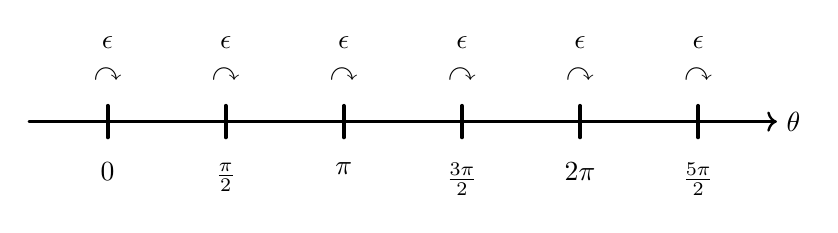
\begin{tikzpicture}[line join = round, line cap = round]
		\coordinate (a) at (0.0,0.8);
		\coordinate (b) at (0.0,-0.4);
		\coordinate (l) at (-1,0);
		\coordinate (m0) at (0,0);
		\tick{(m0)};
		\coordinate[label=above:{$\epsilon$}, label=below:{$\curvearrowright$}] (m0a) at ($(m0) + (a)$);
		\coordinate[label=below:{$0$}] (m0b) at ($(m0) + (b)$);
		\coordinate (m1) at (1.5,0);
		\tick{(m1)};
		\coordinate[label=above:{$\epsilon$}, label=below:{$\curvearrowright$}] (m1a) at ($(m1) + (a)$);
		\coordinate[label=below:{$\frac{\pi}{2}$}] (m1b) at ($(m1) + (b)$);
		\coordinate (m2) at (3,0);
		\tick{(m2)};
		\coordinate[label=above:{$\epsilon$}, label=below:{$\curvearrowright$}] (m2a) at ($(m2) + (a)$);
		\coordinate[label=below:{$\pi$}] (m2b) at ($(m2) + (b)$);
		\coordinate (m3) at (4.5,0);
		\tick{(m3)};
		\coordinate[label=above:{$\epsilon$}, label=below:{$\curvearrowright$}] (m3a) at ($(m3) + (a)$);
		\coordinate[label=below:{$\frac{3\pi}{2}$}] (m3b) at ($(m3) + (b)$);
		\coordinate (m4) at (6.0,0);
		\tick{(m4)};
		\coordinate[label=above:{$\epsilon$}, label=below:{$\curvearrowright$}] (m4a) at ($(m4) + (a)$);
		\coordinate[label=below:{$2\pi$}] (m4b) at ($(m4) + (b)$);
		\coordinate (m5) at (7.5,0);
		\tick{(m5)};
		\coordinate[label=above:{$\epsilon$}, label=below:{$\curvearrowright$}] (m5a) at ($(m5) + (a)$);
		\coordinate[label=below:{$\frac{5\pi}{2}$}] (m5b) at ($(m5) + (b)$);
		\coordinate[label=right:{$\theta$}] (r) at (8.5,0);
		\draw [->,color=black,line width=0.3mm] (l)--(r);
		\end{tikzpicture}
		\caption{\it The dynamics $\theta^\epsilon_n$ for $\epsilon=0$ has fixed points at $0\,\mbox{\rm mod}\,\frac{\pi}{2}$ and therefore has many invariant intervals. However, for $\epsilon>0$ the dynamics crosses the fixed points by steps of size $\epsilon$ to the right.}
		\label{fig:theta}
	\end{center}
\end{figure}



%%%%%%%%%%%%%%%%%%%%%%%%%%%%%%%%%%
\section{Dyson-Schmidt variables and renewal processes}
\label{sec:Dyson-Schmidt}

The Dyson-Schmidt variable $x^\epsilon_n\in\RM$ for $n\in\frac{1}{2}\ZM$ associated to the Pr\"ufer phases is defined by
%
$$
x^\epsilon_n 
\;:=\; 
-\,
\cot(\theta^\epsilon_n)\,.
$$
%
This establishes an orientation preserving bijection of every interval $[k\pi,(k+1)\pi)$ with $k\in\ZM$ to $\overline{\RM}=\RM\cup\{\infty\}$, with the central point $(k+\frac{1}{2})\pi$ being mapped to $0$. Then~\eqref{eq:Q-D-theta} becomes for $n\in\ZM$ and $n'=n-\frac{1}{2}$
%
\begin{equation}\label{eq:Q-D-x}
	x^\epsilon_n
	\;:=\;
	-(R^\epsilon_{n}\cdot (-x^\epsilon_{n'}))
\:=\;
Q^\epsilon_{n}\cdot x^\epsilon_{n'}
	\;,
	\qquad
	x^\epsilon_{n'}
	\;:=\;
	D_{n}\cdot x^\epsilon_{n-1}
	\;,
\end{equation}
%
where the dot $\cdot$ denotes the standard M\"obius action and 
%
$$
Q^\epsilon_{n}
\;:=\;
\begin{pmatrix}
1 & 0 \\ 0 & -1
\end{pmatrix}
R^\epsilon_{n}
\begin{pmatrix}
1 & 0 \\ 0 & -1
\end{pmatrix}
\;,
$$
%
namely $Q^\epsilon_{n}$ is obtained from $R^\epsilon_{n}$ by flipping the signs on the off-diagonals. Due to the explicit forms of $Q^\epsilon_{n}$ and $D_{n}$, the action here becomes
%
\begin{equation}\label{eq:Q-D-explicit}
	x^\epsilon_n
	\;=\;
	\frac{(1+\epsilon^2\alpha^{\epsilon}_n)x^\epsilon_{n'}+(a_n{-b_n}-\epsilon\beta^{\epsilon}_n)\epsilon}{1+\epsilon^2\delta^{\epsilon}_n-(a_n{+b_n}+\epsilon\gamma^{\epsilon}_n)\epsilon x^\epsilon_{n'}}
	\;,
	\qquad
	x^\epsilon_{n'}
	\;=\;
	\kappa_n^2 \, x^\epsilon_{n-1}
	\;,
\end{equation}
%
Note that the interval $[k\pi,(k+1)\pi)$ of Pr\"ufer variables contains two fixed points $k\pi$ and $(k+\frac{1}{2})\pi$ of the dynamics generated by $D_\kappa$, so that one copy $\overline{\RM}$ of the Dyson-Schmidt variable also contains two such fixed points $0$ and $\infty$. The random dynamics on the two half-axis $(-\infty,0)\cup\{\infty\}$ and $[0,\infty)$ is essentially the same, up to flipping the sign of $b_n$, swapping $\alpha^\epsilon_n$ for $\delta^\epsilon_n$ and $\beta^\epsilon_n$ for $-\gamma^\epsilon_n$, as well as changing $\kappa_n$ to $\kappa_n^{-1}$. Indeed, the bijective orientation preserving map $x \in(-\infty,0)\cup\{\infty\}\mapsto -x^{-1}\in[0,\infty)$ identifies these intervals and, moreover,
%
$$
Q^\epsilon_n \cdot (-x^{-1}) 
\,=\,
-\left[\frac{(1+\epsilon^2\delta^\epsilon_n)x + (a_n+b_n+\epsilon\gamma^\epsilon_n)\epsilon}{1+\epsilon^2\alpha^\epsilon_n - (a_n-b_n-\epsilon\beta^\epsilon_n)\epsilon x}\right]^{-1}\,, 
\quad 
D_{n} \cdot (-x^{-1}) 
\,=\, 
-\,\left[\kappa_n^{-2}x\right]^{-1}\,.
$$
%
As all estimates making use of the constants $C_1$, $C_2$, $C_3$ and $\mathbb{E}(\log(\kappa)^2)$ are invariant under the above swapping, it is sufficient to analyze the random dynamics on $[0,\infty)$. On this interval, it will be useful to take the logarithm because, at least at $\epsilon=0$, one has
%
\begin{equation}\label{eq:log}
	\log(x^0_{n+1})
	\;=\;
	\log(x^0_{n})\;+\;2\,\log(\kappa_n)
	\;=\;
	\log(x^0_{n})\;+\;2\,C_0\,\chi_n
	\;,
\end{equation}
%
where $\chi_n=\frac{1}{C_0}\log(\kappa_n)$ is a centered random variable satisfying $-1 \leq \chi_n \leq 1$ almost surely. Hence $\log(x^0_{n})$ is a random walk on $\RM$. It will be shown in the next two sections that in this logarithmic representation the random walk roughly has to go from $\log(\epsilon)$ to $-\log(\epsilon)$, which in expectation takes of order of $\log(\epsilon)^2$ time steps. This provides an intuitive understanding for the behavior in Theorems~\ref{theo:hopping} and \ref{theo:SSH}. Controlling the $\epsilon$-dependent perturbations is quite delicate and the main technical endeavor of this work.

\vspace{.2cm}

The outcome will be bounds for the r.h.s. of~\eqref{eq:IDOS-Birkhoff}. In order to control the rotation number, it is useful to look at the order statistics of the following set of random variables
%
\begin{equation}\label{stat:passages}
	\big\lbrace N \in \mathbb{N} \,:\, x^\epsilon_{N-1} < 0 \leq x^\epsilon_{N} \mbox{ or }   x^\epsilon_{N} < 0 \leq x^\epsilon_{N-1} \big\rbrace\,,
\end{equation}
%
which will be denoted by the random increasing times $N^\epsilon_{(1)}<N^\epsilon_{(2)}<N^\epsilon_{(3)}<...$. These are the random passage times over the two points $0$ and $\infty$ (which are fixed points of the action induced by $D^0_{n}$, so without $\epsilon$-perturbation). Recall that the two conditions in~\eqref{stat:passages} are realized in an alternating manner. For sake of concreteness, let us fix the initial condition $x_0^\epsilon\in (-\infty,0)\cup\{\infty\}$ such that for all $k$ one has $x^\epsilon_{N^\epsilon_{(2k)}-1} < 0 \leq x^\epsilon_{N^\epsilon_{(2k)}}$ and $x^\epsilon_{N^\epsilon_{(2k+1)}} < 0 \leq x^\epsilon_{N^\epsilon_{(2k+1)}-1}$.  The (random) differences $N^\epsilon_{(k+1)}-N^\epsilon_{(k)}$ are the durations of the passages of $x$ through the intervals $[0,+\infty)$ and $\overline{\mathbb{R}} \backslash [0,+\infty)$. Clearly, these quantities depend on the precise value of the initial condition $x_0^\epsilon$ and therefore they are not identically distributed (nor independent). To circumvent this difficulty, two independent and identically distributed families of random dynamical processes $\widehat{x}^\epsilon_k=(\widehat{x}^\epsilon_{k,n})_{n\geq 0}$ and $\widetilde{x}^\epsilon_k=(\widetilde{x}^\epsilon_{k,n})_{n\geq 0}$ on $[0,\infty)$ will be constructed in the two following sections, providing lower and upper bounds on the original process respectively. Note that these processes will not exactly correspond to the notations $\widehat{\theta}^\epsilon_n$ and $\widetilde{\theta}^\epsilon_n$ in~\eqref{stat:order}. They will obey almost surely  that for all $k \in \mathbb{N}$ and then all $n \in \lbrace 0,1,\dots,N^\epsilon_{(k+1)} - N^\epsilon_{(k)}-1\rbrace$
%
\begin{align}\label{stat:slower-faster}
	\widehat{x}_{k,n}^\epsilon\,\leq\, x^\epsilon_{N^\epsilon_{(k)} + n}\, \leq\, \widetilde{x}_{k,n}^\epsilon
	\qquad\mbox{or}\qquad
	\widehat{x}_{k,n}^\epsilon\,\leq\, -\big(x^\epsilon_{N^\epsilon_{(k)} + n}\big)^{-1}\, \leq\, \widetilde{x}_{k,n}^\epsilon
\end{align}
%
and furthermore, for the next step
%
\begin{align}\label{stat:slower-faster-bis}
	\widetilde{x}^\epsilon_{k,N^\epsilon_{(k+1)} - N^\epsilon_{(k)}} \,= \,\infty\,.
\end{align}
%
Note that the left condition in~\eqref{stat:slower-faster} always applies during passages through $(0,\infty)$ and the right condition for passages through $(-\infty,0)$. Also note that the constructed comparison processes are only constrained  on the first $N^\epsilon_{(k+1)} - N^\epsilon_{(k)}$ times. Associated to these two families of processes, there are now two families of random passage times
%
\begin{align}\label{eq-T^}
	\widehat{T}^\epsilon_k \;:=\; \inf\lbrace n \in \mathbb{N}_0 \,:\, \widehat{x}^\epsilon_{k,n} = \infty\rbrace\,,
	\qquad 
	\widetilde{T}^\epsilon_k\;:=\; \inf\lbrace n \in \mathbb{N}_0 \,:\, \widetilde{x}^\epsilon_{k,n} = \infty\rbrace\,.
\end{align}
%
Then~\eqref{stat:slower-faster} and~\eqref{stat:slower-faster-bis} imply that a.s. $\widetilde{T}^\epsilon_k \leq N^\epsilon_{(k+1)} - N^\epsilon_{(k)} \leq \widehat{T}^\epsilon_k$. Furthermore, by construction the families $(\widehat{T}^\epsilon_k)_{k\geq 0}$ and $(\widetilde{T}^\epsilon_k)_{k\geq 0}$ are i.i.d. random variables. As these are interarrival times~\cite{GS}, both families specify a renewal process, given by
%
$$
\widehat{P}^\epsilon_N 
\;:=\; 
\max\Big\lbrace K \in \mathbb{N} \,:\, \sum_{k=1}^K \widehat{T}^\epsilon_k \leq N\Big\rbrace\,,
\qquad 
\widetilde{P}^\epsilon_N 
\;:=\; 
\max\Big\lbrace K \in \mathbb{N} \,:\, \sum_{k=1}^K \widetilde{T}^\epsilon_k \leq N\Big\rbrace\,.
$$
%
This can be interpreted as the number of times the slower or faster process has passed through the interval $[0,+\infty)$. Each such passage corresponds to a passage of the Pr\"ufer variables through $[k\frac{\pi}{2},(k+1)\frac{\pi}{2})$. Thus it follows that
%
$$
\frac{\pi}{2}\big(\widehat{P}^\epsilon_N - 1\big) 
\;\leq\; 
\theta^\epsilon_N 
\;\leq\; 
\frac{\pi}{2}\big(\widetilde{P}^\epsilon_N + 1\big)
$$
%
a.s. for $N \in \mathbb{N}_0$ and $\theta^\epsilon_0 \in \left[-\frac{\pi}{2},\frac{\pi}{2}\right)$. Finally, the elementary renewal theorem~\cite{GS} yields
%
\begin{gather}\label{ineq:slower-faster}
	\frac{1}{2\,\mathbb{E}(\widehat{T}_1^\epsilon)} 
	\;=\; 
	\lim_{N \to \infty} \frac{\widehat{P}^\epsilon_N}{2\,N} 
	\;\leq\; 
	\lim_{N \to \infty} \frac{1}{N}\frac{\mathbb{E}(\theta^\epsilon_N)}{\pi} 
	\;\leq\; 
	\lim_{N \to \infty} \frac{\widetilde{P}^\epsilon_N}{2\,N} 
	\;=\; 
	\frac{1}{2\,\mathbb{E}(\widetilde{T}_1^\epsilon)}\,.
\end{gather}
%
The next two sections will provide the proof of the next result, which by~\eqref{ineq:slower-faster} directly implies Theorems~\ref{theo:hopping} and~\ref{theo:SSH} (since $\EM(L_\sigma)$ is eqaul to $2$ and $2L$ respectively), actually under slightly weaker hypothesis than stated there.

%%%%%%%%%%%%%%%%%%%%%%%%%%%%%%%%%%%%%%%%%%%%%%%%
\begin{proposition}\label{prop:T}
Given a family of random matrices of the form~\eqref{eq:factorization}, suppose that the above Hypothesis hold and the random variables $(\kappa_n)_{n\geq 0}$ are independent with $\EM(\log(\kappa_n)^2)$ independent of $n$. Then
%
$$
\frac{1}{\mathbb{E}(\widehat{T}_1^\epsilon)} 
\;=\;
\frac{\EM(\log(\kappa_0)^2)}{\log(\epsilon)^2}\,\big(1+\Oo(|\log(\epsilon)|^{-1})\big) 
\;,
\qquad
\frac{1}{\mathbb{E}(\widetilde{T}_1^\epsilon)} 
\;=\;
\frac{\EM(\log(\kappa_0)^2)}{\log(\epsilon)^2}\,\big(1+\Oo(|\log(\epsilon)|^{-1})\big) 
\;.
$$
%
\end{proposition}
%%%%%%%%%%%%%%%%%%%%%%%%%%%%%%%%%%%%%%%%%%%%%%%%

%%%%%%%%%%%%%%%%%%%%%%%%%%%%%%%%%%%%%%%%%%%
\section{Lower bound on the rotation number}
\label{sec:lower}

The first task of this section is to construct the slower comparison process satisfying the first inequality of~\eqref{stat:slower-faster} for $k=1$ which is sufficient due to~\eqref{ineq:slower-faster}. To improve readability from this point on, we will suppress the indices $\epsilon$, $\sigma$, $n$, etc., as long as no confusion can arise. Let us start by providing some basic properties of the dynamics, such as the following observation.

%%%%%%%%%%%%%%%%%%%%%%%%%%%%%%%%%%%%%%%%%%%%%%%%
\begin{lemma}
\label{lemma:Q-lower}
For each realization and $\epsilon$ small enough, $x \in [0,\infty)$ and $Q \cdot x \geq 0$ imply $Q \cdot x \geq x$.
\end{lemma}
%%%%%%%%%%%%%%%%%%%%%%%%%%%%%%%%%%%%%%%%%%%%%%%%


\noindent {\bf Proof.} The main Hypothesis implies for $x \in [0,1]$ the estimates
%
$$
Q \cdot x
\, =\, 
\tfrac{(1+\epsilon^2\alpha)x + (a-b-\epsilon\beta)\epsilon}{1+\epsilon^2\delta - (a+b+\epsilon\gamma)\epsilon x}
\,\geq\,
x\,\tfrac{1+\epsilon^2\alpha + (a-b-\epsilon\beta)\frac{\epsilon}{x}}{1+\epsilon^2\delta} 
\,\geq \,
x\,\tfrac{1+C_1\,\epsilon-2\,C_3\,\epsilon^2}{1+C_3\,\epsilon^2}\,, 
$$
%
while for $x \in (1,\infty)$
%
$$
Q \cdot x
\,\geq\,
x\,\tfrac{1+\epsilon^2\alpha}{1+\epsilon^2\delta - (a+b+\epsilon\gamma)\epsilon x}
\,\geq\,
x\,\tfrac{1+\epsilon^2\alpha}{1+\epsilon^2\delta - (a+b+\epsilon\gamma)\epsilon }
\, \geq\, 
x\,\tfrac{1-C_3\,\epsilon^2}{1-C_1\,\epsilon+2\,C_3\,\epsilon^2}
\,.
$$
%
In both cases the statement directly follows. (Note that the lemma can also be deduced from~\eqref{eq:Q-S^1}.)
\hfill $\Box$

\vspace{.2cm}

The following lemma states more properties of the given action, and relies on the quantities
%
$$
\widehat{x}_-
\;:=\;
\tfrac{C_1\,\epsilon}{2}
\;,
\qquad
\widehat{x}_c
\;:=\;
\tfrac{C_1\epsilon}{2}(e^{-2C_0}+1)
\;,
\qquad
\widehat{x}_+
\;:=\;
\tfrac{2\,e^{2C_0}}{C_1\epsilon}
\;.
$$
%
These points and the lemma itself are graphically illustrated in the left part of Fig.~\ref{fig:slower}.

\begin{figure}
	\begin{center}
		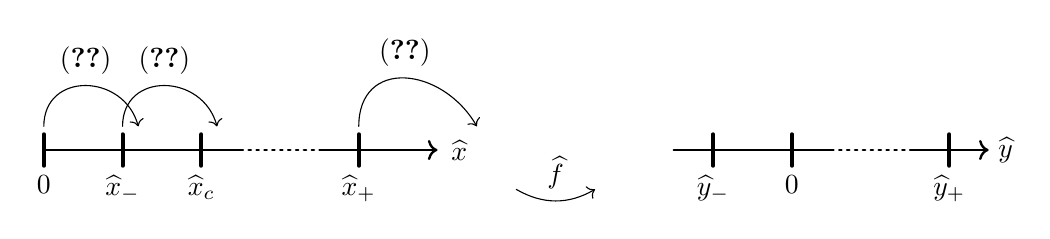
\begin{tikzpicture}[line join = round, line cap = round]
		\coordinate (a) at (0.0,0.3);
		\coordinate (b) at (0.0,-0.2);
		\coordinate (bb) at (0.0,-0.8);
		\coordinate (r) at (0.2,0.0);
		\coordinate (l0) at (-6.5,0);
		\tick{(l0)};
		\coordinate (l0a) at ($(l0) + (a)$);
		\coordinate[label=below:{$0$}] (l0b) at ($(l0) + (b)$);
		\coordinate (l1) at (-5.5,0);
		\tick{(l1)};
		\coordinate (l1a) at ($(l1) + (a)$);
		\coordinate (l1ar) at ($(l1) + (a) + (r)$);
		\draw[->] (l0a) to[out=90, in=105, looseness=1.5] node[midway,above,inner sep=4pt] {\eqref{stat:slower-start}} (l1ar);
		\coordinate[label=below:{$\widehat{x}_-$}] (l1b) at ($(l1) + (b)$);
		\coordinate (l2) at (-4.5,0);
		\tick{(l2)};
		\coordinate (l2ar) at ($(l2) + (a) + (r)$);
		\draw[->] (l1a) to[out=90, in=105, looseness=1.5] node[midway,above,inner sep=4pt] {\eqref{stat:slower-between}} (l2ar);
		\coordinate[label=below:{$\widehat{x}_c$}] (l2b) at ($(l2) + (b)$);
		\coordinate (l3) at (-4,0);
		\coordinate (l4) at (-3,0);
		\coordinate (l5) at (-2.5,0);
		\tick{(l5)};
		\coordinate (l5a) at ($(l5) + (a)$);
		\coordinate[label=below:{$\widehat{x}_+$}] (l5b) at ($(l5) + (b)$);
		\coordinate (lr) at (-1.5,0);
		\coordinate[label=left:{$\widehat{x}$}] (lrr) at (-1,0);
		\coordinate (lrra) at ($(lrr) + (a)$);
		\draw[->] (l5a) to[out=90, in=120, looseness=1.5] node[midway,above,inner sep=4pt] {\eqref{stat:slower-end}} (lrra);
		\draw [-,color=black,line width=0.3mm] (l0)--(l3);
		\draw [-,color=black,dotted,line width=0.3mm] (l3)--(l4);
		\draw [->,color=black,line width=0.3mm] (l4) -- (lr);
		\coordinate (ml) at (-0.5,-0.5);
		\coordinate (mr) at (0.5,-0.5);
		\draw[->] (ml) to[bend right] node[midway,above,inner sep=4pt] {$\widehat{f}$} (mr);
		\coordinate (rl) at (1.5,0);
		\coordinate (r1) at (2,0);
		\tick{(r1)};
		\coordinate[label=below:{$\widehat{y}_-$}] (r1b) at ($(r1) + (b)$);
		\coordinate (r2) at (3,0);
		\tick{(r2)};
		\coordinate[label=below:{$0$}] (r2b) at ($(r2) + (b)$);
		\coordinate (r3) at (3.5,0);
		\coordinate (r4) at (4.5,0);
		\coordinate (r5) at (5,0);
		\tick{(r5)};
		\coordinate[label=below:{$\widehat{y}_+$}] (r5b) at ($(r5) + (b)$);
		\coordinate[label=right:{$\widehat{y}$}] (rr) at (5.5,0);
		\draw [-,color=black,line width=0.3mm] (rl)--(r3);
		\draw [-,color=black,dotted,line width=0.3mm] (r3)--(r4);
		\draw [->,color=black,line width=0.3mm] (r4) -- (rr);
		\end{tikzpicture}
		\caption{\it The arrows on the left part illustrate properties of the original Dyson-Schmidt dynamics on $(0,\infty)$ as stated in {\rm Lemma~\ref{lemma:slower}}. The right part illustrates the notations after the logarithmic transformation $\widehat{f}$ to $\mathbb{R}$.}
		\label{fig:slower}
	\end{center}
\end{figure}
	
%%%%%%%%%%%%%%%%%%%%%%%%%%%%%%%%%%%%%%%
\begin{lemma}\label{lemma:slower}
For each realization, one has
\begin{alignat}{3}
	& x \,\in\, [0,\infty)  &\qquad \Longrightarrow \qquad & Q \cdot (D \cdot x) \,\notin\, [0,\widehat{x}_-)\,,
	\label{stat:slower-start}\\
	& x \,\in\, [\widehat{x}_-,\infty)  &\qquad \Longrightarrow \qquad  &  Q \cdot (D \cdot x) \,\notin\, [0,\widehat{x}_c)\,,
	\label{stat:slower-between}\\
	& Q \cdot (D \cdot x) \,\in\, [0,\infty)  &\qquad \Longrightarrow \qquad  & x \,\notin\, [\widehat{x}_+,\infty)\,.
	\label{stat:slower-end}
\end{alignat}
\end{lemma}
%%%%%%%%%%%%%%%%%%%%%%%%%%%%%%%%%%%%%%%

\noindent {\bf Proof.} For~\eqref{stat:slower-start}, first note that $x \in [0,\infty)$ implies $D \cdot x \in [0,\infty)$. By combining~\eqref{eq:Q-S^1} and the order-preserving property~\eqref{stat:order}, then nonnegative $Q \cdot (D \cdot x)$ obey, due to~\eqref{eq:Q-D-explicit} and the Hypothesis,
%
$$
Q \cdot (D \cdot x) 
\;\geq \;
Q \cdot 0 
\;=\; 
\tfrac{(a-b-\epsilon\beta)\epsilon}{1+\epsilon^2\delta} 
\;\geq\; 
\tfrac{(C_1-C_3\epsilon)\epsilon}{1+C_3\epsilon^2} 
\;\geq\; 
\tfrac{C_1\,\epsilon}{2}
\;=\;
\widehat{x}_-
\;.
$$
%
For the proof of~\eqref{stat:slower-between} let us use that, if $x \in [\widehat{x}_-,\infty)$, then clearly $D \cdot x \geq e^{-2C_0}\widehat{x}_-$. Similarly to the proof of~\eqref{stat:slower-start}, nonnegative $Q \cdot (D \cdot x)$ then obey
$$
Q \cdot (D \cdot x) 
\;\geq\; 
Q \cdot \tfrac{e^{-2C_0}C_1\epsilon}{2} 
\;\geq\; 
\tfrac{(1-C_3\epsilon^2)\frac{e^{-2C_0}C_1\epsilon}{2} + (C_1-C_3\epsilon)\epsilon}{1+C_3\epsilon^2 - (C_1-C_3\epsilon)\frac{e^{-2C_0}C_1\epsilon^2}{2}} 
\;\geq\; 
(e^{-2C_0} + 1)\tfrac{C_1\epsilon}{2}
\;=\;\widehat{x}_c
\;.
$$
%
Finally let us verify~\eqref{stat:slower-end} by contraposition. If $x \in [\widehat{x}_+,\infty)$, then clearly $D \cdot x \geq e^{-2C_0}\widehat{x}_+=\tfrac{2}{C_1\epsilon}$. Then the order-preserving property~\eqref{stat:order} implies that $Q \cdot (D \cdot x) \notin [0,\infty)$, since as in the proof of~\eqref{stat:slower-start} it holds that 
%
$$
0 
\;>\; 
Q \cdot \infty 
\;\geq \;
Q \cdot (D \cdot x) 
\;\geq\; 
Q \cdot \tfrac{2}{C_1\epsilon} 
\;\geq\; 
\tfrac{(1-C_3\epsilon^2)\frac{2}{C_1\epsilon} + (C_1-C_3\epsilon)\epsilon}{1+C_3\epsilon^2 - (C_1-C_3\epsilon)\frac{2}{C_1}}
\;,
$$ 
%
which is also negative.
\hfill $\Box$

\vspace{.2cm}

Now a new process $\widehat{x}=(\widehat{x}_n)_{n\geq 0}$ is constructed by setting $\widehat{x}_0 = 0$, $\widehat{x}_1=\widehat{x}_-$ and for $n\geq 1$
%
$$
\widehat{x}_{n+1} 
\;=\; 
\begin{cases}
\widehat{x}_c \;,&\text{ if } \widehat{x}_n \leq \widehat{x}_-\;,\\
D_n \cdot \widehat{x}_n \;,&\text{ if } \widehat{x}_n \in (\widehat{x}_-,\widehat{x}_+)\;,
\\
\infty\;, &\text{ else, so if } \widehat{x}_n \geq  \widehat{x}_+\,.
\end{cases}
$$
%
Comparing with~\eqref{eq:Q-D-x}, the main case $\widehat{x}_{n+1}=D_n \cdot \widehat{x}_n$ of this process merely omits the action of $Q_n$ for $n\geq 2$. Let us now argue why this process satisfies the first inequality in~\eqref{stat:slower-faster}. Indeed, omitting the action of $Q_n$ slows the process down because of the order-preserving property~\eqref{stat:order} and Lemma~\ref{lemma:Q-lower}. Carefully analyzing the first case in the definition of $\widehat{x}_{n+1}$ in combination with~\eqref{stat:slower-start} and~\eqref{stat:slower-between} shows that a.s. $\widehat{x}_n \leq x_{N_{(1)} + n}$ for all $n \in \lbrace 0,1,\dots,N_{(2)} - 1 - N_{(1)}\rbrace$, that is, as long as $x_{N_{(1)} + n} \in [0,\infty)$. Moreover, by~\eqref{stat:slower-end} it is impossible that $\widehat{x}_n = \infty$ for $n \in \lbrace 3,4,\dots,N_{(2)} - 1 - N_{(1)}\rbrace$, as this would imply $x_{N_{(1)} + n-1} < \widehat{x}_+ \leq \widehat{x}_{n-1}$. Conversely, as a.s. $\widehat{x}_{\widehat{T}_1} = \infty$, then indeed $N_{(2)} - N_{(1)} \leq \widehat{T}_1$. 

\vspace{.2cm}

Now let us come to the second task, namely analyze the $\epsilon$-dependence of $\big(\EM(\widehat{T}_1)\big)^{-1}$ and thereby prove the first statement of Proposition~\ref{prop:T}. Similar as in~\eqref{eq:log}, it will be advantageous to pass to a shifted logarithm of the Dyson-Schmidt variables, via the map $\widehat{f}:(0,\infty)\to \RM$ given by 
%
$$
\widehat{f}(x)
\;:=\;
\frac{1}{2C_0}\,\log\Big(\frac{x}{\widehat{x}_c}\Big)
\;.
$$
%
By construction, $\widehat{f}(\widehat{x}_c) = 0$. Furthermore, for $n$ such that $\widehat{x}_{n+1}<\infty$, let us introduce 
%
$$
\widehat{y}_n
\;:=\;
\widehat{f}(\widehat{x}_{n+2})
\;,
\qquad
\widehat{y}_-\;:=\;\widehat{f}(\widehat{x}_-)
\;,
\qquad
\widehat{y}_+\;:=\;\widehat{f}(\widehat{x}_+)
\;,
$$
%
and the stopping time
%
$$
\widehat{T}_{-,+}
\;:= \;
\inf\big\{ n \in \mathbb{N} \,:\, 
\widehat{y}_n\notin (\widehat{y}_-,\widehat{y}_+) 
\big\}\,.
$$
%
Again these objects are illustrated in Fig.~\ref{fig:slower}. As long as $n \leq \widehat{T}_{-,+}$, it holds that
%
\begin{gather}\label{eq:y-slower}
	\widehat{y}_n 
	\;=\; 
	\tfrac{1}{2C_0}\,\log\Big(\frac{\widehat{x}_{n+2}}{\widehat{x}_c}\Big)
	\;=\; 
	\tfrac{1}{2C_0}\log\Big(\frac{D^n \cdot \widehat{x}_2}{\widehat{x}_c}\Big)
	\;=\; 
	\tfrac{1}{2C_0}\log\Big(\prod_{j=N_{(1)}+1}^{N_{(1)}+n} \kappa_j^2\Big) 
	\;=\; 
	\sum_{j=N_{(1)}+1}^{N_{(1)}+n} \chi_j\,,
\end{gather}
%
namely $ \widehat{y}_n $ is a centered random walk starting at $\widehat{y}_0=0$. The following two lemmata recollect properties about these newly introduced quantities.

%%%%%%%%%%%%%%%%%%%%%%%%%%%%%%%%%%%%%%%
\begin{lemma}\label{lemma:slower-y-lims}
$\widehat{y}_- \in (-\infty,0)$ is independent of $\epsilon$ and $\lim_{\epsilon \to 0} \frac{\widehat{y}_+}{-\log(\varepsilon)} = \frac{1}{C_0}$.
\end{lemma}
%%%%%%%%%%%%%%%%%%%%%%%%%%%%%%%%%%%%%%%

\noindent\textbf{Proof.} The explicit expressions
%
$$
\widehat{y}_- \,=\, -\tfrac{1}{2\,C_0}\,\log(1+e^{-2\,C_0})\;,
\qquad
\widehat{y}_+ \,=\, \tfrac{1}{2\,C_0}\big(2\log\big(\tfrac{2}{C_1\,\epsilon}\big) -\log(1+e^{-2\,C_0})\big) +1
\,,
$$
%
immediately imply the claims.
\hfill $\square$

%%%%%%%%%%%%%%%%%%%%%%%%%%%%%%%%%%%%%%%
\begin{lemma}\label{lemma:E-T-slower}
$\mathbb{E}(\widehat{T}_{-,+} ) < +\infty$
\end{lemma}
%%%%%%%%%%%%%%%%%%%%%%%%%%%%%%%%%%%%%%%

\noindent\textbf{Proof.}
Since the cumulative distribution function of $\chi$ is right-continuous and $\mathbb{P}(\{\chi > 0\}) > 0$, there exists some $\ell \in (0,1]$ such that $ \widehat{p}:=\mathbb{P}(\{\chi \geq \ell\})$ satisfies  $\widehat{p} > 0$. Denoting $\widehat{E} := \lceil\frac{\widehat{y}_+-\widehat{y}_-}{\ell}\rceil$, the random variable 
%
$$
\widehat{N}
\; := \;
\min\lbrace n \in \mathbb{N} \,:\, \chi_{(n-1)\widehat{E} + 1} \geq \ell\;,\; \chi_{(n-1)\widehat{E} + 2} \geq \ell\;, \dots,\; \chi_{n\widehat{E}} \geq \ell \rbrace
\;,
$$ 
%
is then geometrically distributed with success probability $\widehat{p}^{\widehat{E}}$. In particular, one has $\mathbb{E}(\widehat{N}) < \infty$. Moreover, the inequality $\widehat{T}_{-,+} < \widehat{E}\,\widehat{N}$ holds a.s. by construction. Therefore one deduces  $\mathbb{E}(\widehat{T}_{-,+}) < \widehat{E}\,\mathbb{E}(\widehat{N}) < \infty$.
\hfill $\square$

\vspace{.2cm}



In order to connect the two stopping times $\widehat{T}_{-,+}$ and $\widehat{T}_1$, one further random variable will be introduced. Suppose that $\widehat{T}_{-,+} = m$ for some $m \in \mathbb{N}$, and $\widehat{y}_{\widehat{T}_{-,+}}\leq\widehat{y}_-$, then let us introduce the at $m+1$ reinitialized stopping time as in~\eqref{eq-T^} by
%
$$
\widehat{T}^{(m)}_1 
\;:=\; 
\inf\big\{ n \in \mathbb{N} \,:\, \widehat{x}_{m+1+n} = \infty \big\}
\;.
$$
%
It then clearly follows that $\widehat{T}_1 = m + 1 + \widehat{T}^{(m)}_1$, provided that $\widehat{T}_{-,+} = m$ and $\widehat{y}_{m}\leq\widehat{y}_-$. Now the Markov property allows to compute the conditional expectations
%
$$
\mathbb{E}\big(\widehat{T}^{(m)}_1 \,\big|\, \widehat{y}_{m} \leq \widehat{y}_-\,,\;\; \widehat{T}_{-,+}=m\big) 
\;=\; 
\mathbb{E}(\widehat{T}_1)
\,,\qquad
\mathbb{E}\big(\widehat{T}_1 \,\big|\, \widehat{y}_{\widehat{T}_{-,+}} \geq \widehat{y}_+\big)
\;=\; 
\mathbb{E}\big(\widehat{T}_{-,+} + 3 \,\big|\, \widehat{y}_{\widehat{T}_{-,+}} \geq \widehat{y}_+\big)
\;,
$$
%
where the $3$ stems from an index shift by $2$ when then processes is started and $1$ additional step at the end. As by construction $\mathbb{P}\big(\{\widehat{y}_{\widehat{T}_{-,+}}\in(\widehat{y}_-,\widehat{y}_+)\}\big)=0$ and as by Lemma~\ref{lemma:E-T-slower} one has $\widehat{T}_{-,+}<\infty$ a.s., it follows that
%
\begin{align*}
\begin{aligned}
	\mathbb{E}(\widehat{T}_1) 
	&\;=\; \mathbb{E}\big(\widehat{T}_1 \,\big|\, \widehat{y}_{\widehat{T}_{-,+}} \geq \widehat{y}_+\big)\,\mathbb{P}\big(\big\{\widehat{y}_{\widehat{T}_{-,+}} \geq \widehat{y}_+\big\}\big) 
	\\
	& \qquad + \sum_{m=0}^{\infty} \mathbb{E}\big(\widehat{T}_1 \,\big|\, \widehat{y}_m \leq \widehat{y}_-\,, \widehat{T}_{-,+}  = m\big)\,\mathbb{P}\big(\big\{\widehat{y}_m \leq \widehat{y}_-\,, \widehat{T}_{-,+}  = m\big\}\big)\\
	&\;=\; \mathbb{P}\big(\big\{\widehat{y}_{\widehat{T}_{-,+}} \geq \widehat{y}_+\big\}\big)\,\mathbb{E}\big(\widehat{T}_1 \,\big|\, \widehat{y}_{\widehat{T}_{-,+}} \geq \widehat{y}_+\big) 
	\\
	& \qquad + \sum_{m=0}^{\infty} \mathbb{P}\big(\big\{\widehat{y}_m \leq \widehat{y}_-\,, \widehat{T}_{-,+}  = m\big\}\big)\mathbb{E}\big(m + 1 + \widehat{T}^{(m)}_1 \,\big|\, \widehat{y}_{m} \leq \widehat{y}_-\,, \widehat{T}_{-,+}  = m\big)
	\\
	&\;= \;\mathbb{P}\big(\big\{\widehat{y}_{\widehat{T}_{-,+}} \geq \widehat{y}_+\big\}\big)\,\mathbb{E}\big(\widehat{T}_{-,+} + 3 \,\big|\, \widehat{y}_{\widehat{T}_{-,+}} \geq \widehat{y}_+\big)
	\\
	& \qquad + \sum_{m=0}^{\infty} \mathbb{P}\big(\big\{\widehat{y}_m \leq \widehat{y}_-\,, \widehat{T}_{-,+}  = m\big\}\big)\left(\mathbb{E}\big(\widehat{T}_{-,+} \,\big|\, \widehat{y}_{\widehat{T}_{-,+}} \leq \widehat{y}_-\,, \widehat{T}_{-,+}  = m\big) + 1 + \mathbb{E}(\widehat{T}_1)\right)
	\\
	&\;=\; \mathbb{E}(\widehat{T}_{-,+} )\, +\, 3\,\mathbb{P}\big(\big\{\widehat{y}_{\widehat{T}_{-,+}} \geq \widehat{y}_+\big\}\big)\, +\, \left(1-\mathbb{P}\big(\big\{\widehat{y}_{\widehat{T}_{-,+}} \geq \widehat{y}_+\big\}\big)\right)\left(1 + \mathbb{E}(\widehat{T}_1)\right)\,,
\end{aligned}
\end{align*}
%
which is equivalent to
%
\begin{gather}\label{ineq:slower}
	\big(\EM(\widehat{T}_1)\big)^{-1}
	\;=\; \left[\frac{\mathbb{E}(\widehat{T}_{-,+}) + 1}{\mathbb{P}\big(\big\{\widehat{y}_{\widehat{T}_{-,+}} \geq \widehat{y}_+\big\}\big)}\, +\, 2\right]^{-1}\,.
\end{gather}
%
It now remains to compute the probability and the expectation on the r.h.s. of~\eqref{ineq:slower}. This will essentially follow from the optional stopping theorem. It is convenient to define the quantities
%
\begin{align*}
	\widehat{y}'_- &:=\, \mathbb{E}\big(\widehat{y}_{\widehat{T}_{-,+}} \,\big|\, \widehat{y}_{\widehat{T}_{-,+}} \leq \widehat{y}_-\big) \in \left[\widehat{y}_--1,\widehat{y}_-\right]\,,&\quad& \widehat{y}''_- :=\, -\sqrt{\mathbb{E}\big(\widehat{y}^2_{\widehat{T}_{-,+}} \,\big|\, \widehat{y}_{\widehat{T}_{-,+}} \leq \widehat{y}_-\big)} \in \left[\widehat{y}_--1,\widehat{y}_-\right],
	\\
\widehat{y}'_+ &:=\, \mathbb{E}\big(\widehat{y}_{\widehat{T}_{-,+}} \,\big|\, \widehat{y}_{\widehat{T}_{-,+}} \geq \widehat{y}_+\big) \in \left[\widehat{y}_+,\widehat{y}_++1\right]\,,&\quad& \widehat{y}''_+ :=\, \sqrt{\mathbb{E}\big(\widehat{y}^2_{\widehat{T}_{-,+}} \,\big|\, \widehat{y}_{\widehat{T}_{-,+}} \geq \widehat{y}_+\big)} \in \left[\widehat{y}_+,\widehat{y}_++1\right]\,.
\end{align*}
%
Now $\mathbb{E}(\chi) = 0$ implies that both $\widehat{y}_n$ and $\widehat{y}_n^2 - n\mathbb{E}(\chi^2)$ are martingales. As $|\chi| \leq 1$ a.s., both have a.s. bounded increments for times smaller than $\widehat{T}_{-,+} $. More concretely, one has $|\widehat{y}_{n+1} - \widehat{y}_n| \leq 1$ and $|\widehat{y}_{n+1}^2 - (n+1)\mathbb{E}(\chi^2) - \widehat{y}_n^2 + n\mathbb{E}(\chi^2)| \leq 2(\widehat{y}_+-\widehat{y}_-) + 1 + \mathbb{E}(\chi^2)$. Together with $\mathbb{E}(\widehat{T}_{-,+} ) < \infty$ assured by Lemma~\ref{lemma:E-T-slower} this allows to use the optional stopping theorem, and one then finds
%
\begin{gather}\label{eq:slower}
	0 
	\;=\; 
	\mathbb{E}(\widehat{y}_0) 
	\;=\; 
	\mathbb{E}\big(\widehat{y}_{\widehat{T}_{-,+}}\big) 
	\;=\; 
	\widehat{y}'_-\left(1 - \mathbb{P}\big(\big\{ \widehat{y}_{\widehat{T}_{-,+}} \geq \widehat{y}_+ \big\}\big)\right) \,+\, \widehat{y}'_+\,\mathbb{P}\big(\big\{ \widehat{y}_{\widehat{T}_{-,+}} \geq \widehat{y}_+ \big\}\big)\,.
\end{gather}
%
Similarly, $0 = \mathbb{E}\big(\widehat{y}_0^2 - 0 \cdot \mathbb{E}(\chi^2)\big) = \mathbb{E}\big(\widehat{y}^2_{\widehat{T}_{-,+}} - \widehat{T}_{-,+}  \cdot \mathbb{E}(\chi^2)\big)$ again by the optional stopping theorem, which then implies
%
\begin{gather}\label{eq:slower-bis}
	\frac{\mathbb{E}(\chi^2)\,\mathbb{E}(\widehat{T}_{-,+} )}{\mathbb{P}\big(\big\{\widehat{y}_{\widehat{T}_{-,+}} \geq \widehat{y}_+\big\}\big)} 
	\;=\; 
	\frac{\mathbb{E}\big(\widehat{y}^2_{\widehat{T}_{-,+}}\big)}{\mathbb{P}\big(\big\{\widehat{y}_{\widehat{T}_{-,+}} \geq \widehat{y}_+\big\}\big)} 
	\;=\; 
	(\widehat{y}''_+)^2 \,-\, (\widehat{y}''_-)^2 \,+\, \frac{(\widehat{y}''_-)^2}{\mathbb{P}\big(\big\{\widehat{y}_{\widehat{T}_{-,+}} \geq \widehat{y}_+\big\}\big)}\,.
\end{gather}
%
Finally, combining~\eqref{ineq:slower},~\eqref{eq:slower} and~\eqref{eq:slower-bis} yields
%
\begin{align*}
	\big(\EM(\widehat{T}_1)\big)^{-1}
	&\;=\;
	\mathbb{E}(\chi^2)\left[(\widehat{y}''_+)^2 \,-\, (\widehat{y}''_-)^2\, +\, 2\mathbb{E}(\chi^2) \,+\, \frac{(\widehat{y}''_-)^2 + \mathbb{E}(\chi^2)}{\mathbb{P}\big(\big\{\widehat{y}_{\widehat{T}_{-,+}} \geq \widehat{y}_+\big\}\big)}\right]^{-1}\\
	&\;=\; \frac{\mathbb{E}(\chi^2)}{(\widehat{y}''_+)^2}\left[1 \,+\, \frac{\mathbb{E}(\chi^2)(\widehat{y}'_+ - 3\widehat{y}'_-) + \widehat{y}'_+(\widehat{y}''_-)^2}{-\widehat{y}'_-(\widehat{y}''_+)^2}\right]^{-1}\,.
\end{align*}
%
which together with the two statements of Lemma~\ref{lemma:slower-y-lims} implies the first statement of Proposition~\ref{prop:T}.


%%%%%%%%%%%%%%%%%%%%%%%%%%%%%%%%%%%%%%%%%%%%%%%%%%%%%%%%
\section{Upper bound on the rotation number}
\label{sec-Upper}

This section is structured just as the previous one, namely first a faster comparison process satisfying~\eqref{stat:slower-faster-bis} is constructed and then the $\epsilon$-dependence of its expected stopping time is analyzed in order to prove the second statement of Proposition~\ref{prop:T}. It will be useful to introduce the following two supplementary notations:
%
$$
\lambda
\;:=\;
\frac{1}{2C_0\,\big[\log(\tfrac{1}{\epsilon})\big]^2}
\;,
\qquad
\explambda
\;:=\;
e^{2C_0\lambda}
\;.
$$
%
Note that both $\lambda$ and $\explambda$ depend on $\epsilon$. Similar as in Section~\ref{sec:lower}, three reference points $0<\widetilde{x}_-<\widetilde{x}_c<\widetilde{x}_+<\infty$ will be needed w.r.t. which the dynamics has uniform properties schematically described in  Fig.~\ref{fig:faster}. While similar to  Fig.~\ref{fig:slower}, note that the original dynamics now is bounded above by these points, see Lemma~\ref{lemma:faster} below. For its proof, let us start out with a counterpart to Lemma~\ref{lemma:Q-lower}. 

%%%%%%%%%%%%%%%%%%%%%%%%%%%
\begin{lemma}\label{lemma:Q-upper}
There exist $\widetilde{x}_-$ and $\widetilde{x}_+$ depending on $C_0$, $C_2$, $C_3$ and $\epsilon$ such that
%
$$
x \,\in \,[\widetilde{x}_-,\widetilde{x}_+]
\qquad
\Longrightarrow
\qquad
Q \cdot (D \cdot x) \,\leq\, \explambda(D \cdot x)
\;,
$$ 
%
as well as
%
\begin{gather}\label{eq:faster-x-lims}
	\lim_{\epsilon \to 0} \;\frac{\lambda\,\widetilde{x}_-}{\epsilon} 
	\;= \;
	\frac{C_2\,e^{2C_0}}{2C_0}
	\;,
	\qquad
	\lim_{\epsilon \to 0} \;\frac{\epsilon\,\widetilde{x}_+}{\lambda}
	\;= \;
	\frac{2C_0}{C_2\,e^{2C_0}}
	\,.
\end{gather}
%
\end{lemma}
%%%%%%%%%%%%%%%%%%%%%%%%%%%

\noindent\textbf{Proof.}
For $x \in [0,+\infty)$ one can estimate
%
$$
Q \cdot (D \cdot x) 
\;=\; 
\frac{(1+\epsilon^2\alpha)(D \cdot x) + (a-b-\epsilon\beta)\epsilon}{1+\epsilon^2\delta - (a+b+\epsilon\gamma)\epsilon(D \cdot x)} 
\;\leq\; 
\frac{(1+C_3\epsilon^2)(D \cdot x) + (C_2+C_3\epsilon)\epsilon}{1-C_3\epsilon^2 - (C_2+C_3\epsilon)\epsilon(D \cdot x)}
\;.
$$
%
The latter is smaller than or equal to $\explambda(D \cdot x)$ if and only if
%
$$
\explambda(C_2+C_3\epsilon)\epsilon(D \cdot x)^2 - \big(\explambda-1-C_3\epsilon^2(\explambda+1)\big)(D \cdot x) + (C_2+C_3\epsilon)\epsilon 
\;\leq\; 
0\,.
$$
%
Let us equate this to $A(D \cdot x)^2 - B(D \cdot x) + C$, namely set
%
$$
A 
\;:=\; \explambda(C_2+C_3\epsilon)\epsilon
\,,
\qquad 
B 
\;:= \;
\explambda-1-C_3\epsilon^2(\explambda+1)\,,
\qquad 
C 
\;:= \;
(C_2+C_3\epsilon)\epsilon
\,.
$$
%
 Note that $A,B,C \in (0,+\infty)$ for $\epsilon$ small enough. Now let us search for real solutions of the quadratic equation $A(D \cdot x)^2 - B(D \cdot x) + C=0$. They clearly exist whenever $B^2 - 4AC \geq 0$. As
%
\begin{align*}
	\lim_{\epsilon \to 0} \frac{4\,A\,C\,\lambda^2}{B^2\,\epsilon^2} 
	&
	\;=\; 
	\left[\lim_{\epsilon \to 0} \explambda\right]\left[\lim_{\epsilon \to 0} 4\,(C_2+C_3\epsilon)^2\right]\left(\left[\lim_{\epsilon \to 0} \tfrac{\explambda-1}{\lambda}\right] - C_3\left[\lim_{\epsilon \to 0} \tfrac{\epsilon^2}{\lambda}\right]\left[\lim_{\epsilon \to 0} (\explambda+1)\right]\right)^{-2}
	\\
	&
	\;=\; 1 \cdot 4\,C_2^2 \cdot \left(C_0 - C_3 \cdot 0 \cdot 2\right)^{-2} 
	\\
	& 
	\;= \;
	\tfrac{4\,C_2^2}{C_0^2}\,,
\end{align*}
%
and $\frac{\epsilon}{\lambda} = C_0[-\epsilon^{\frac{1}{2}}\log(\epsilon)]^2 \to 0$ for $\epsilon \to 0$, one has $\frac{4AC}{B^2} \in [0,1]$ for $\epsilon$ small enough. Now denote the two real zeroes of the quadratic equation by $x_- \leq x_+$, so $A(D \cdot x)^2 - B(D \cdot x) + C$ then equals $A\left[(D \cdot x)-x_+\right]\left[(D \cdot x)-x_-\right]$. The fact that $\sqrt{1-r} \geq 1-\frac{r}{2}-\frac{r^2}{2} \geq 1-r$ for all $r \in [0,1]$ implies after some algebra that $x_- \leq \frac{(B^2+4AC)C}{B^3}$ and $x_+\geq\frac{B^2-2AC}{AB} $. Hence let us set
%
\begin{align*}
	\widetilde{x}_- 
	&
	\;:=\; 
	e^{2C_0}\,\frac{(B^2+4AC)C}{B^3}
	\;=\;
	\frac{\big[\big(\explambda-1-C_3\epsilon^2(\explambda+1)\big)^2 + 4\explambda(C_2+C_3\epsilon)^2\epsilon^2\big](C_2+C_3\epsilon)\,e^{2C_0}\,\epsilon}{\left(\explambda-1-C_3\epsilon^2\left[\explambda+1\right]\right)^3}
	\,,
	\\
	\widetilde{x}_+ 
	&
	\;:=\;
	e^{-2C_0}\,\frac{B^2-2AC}{AB}
	\;=\;
	\frac{\big(\explambda-1-C_3\epsilon^2(\explambda+1)\big)^2 \,- \,2\,\explambda\,(C_2+C_3\epsilon)^2\,\epsilon^2}{\big(\explambda-1-C_3\epsilon^2(\explambda+1)\big)\,\explambda\,(C_2+C_3\epsilon)\,e^{2C_0}\,\epsilon}\,.
\end{align*}
%
Then, if $x \in [\widetilde{x}_-,\widetilde{x}_+]$, one has due to $e^{-2C_0}x \leq (D \cdot x) \leq e^{2C_0}x$ that $(D \cdot x) \in [e^{-2C_0}\widetilde{x}_-,e^{2C_0}\widetilde{x}_+]\subset[x_-,x_+]$, which by the above implies the first statement. The limits~\eqref{eq:faster-x-lims} follow again from $\frac{\epsilon}{\lambda} = C_0[-\epsilon^{\frac{1}{2}}\log(\epsilon)]^2 \to 0$ and $\frac{\explambda-1}{\lambda} \to 2C_0$ for $\epsilon \to 0$.
\hfill $\square$

\vspace{.2cm}

Let us now complete the left part of Fig.~\ref{fig:faster} by setting
%
$$
\widetilde{x}_c
\;:=\;
e^{2C_0}\,\explambda\,\widetilde{x}_-
\;.
$$
%
The next statement corresponds to Lemma~\ref{lemma:slower}.

\begin{figure}
	\begin{center}
		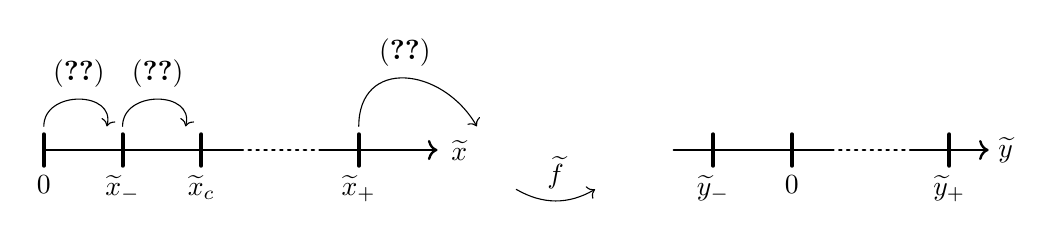
\begin{tikzpicture}[line join = round, line cap = round]
		\coordinate (a) at (0.0,0.3);
		\coordinate (b) at (0.0,-0.2);
		\coordinate (l) at (-0.2,0.0);
		\coordinate (l0) at (-6,0);
		\coordinate (l0) at (-6.5,0);
		\tick{(l0)};
		\coordinate (l0a) at ($(l0) + (a)$);
		\coordinate[label=below:{$0$}] (l0b) at ($(l0) + (b)$);
		\coordinate (l1) at (-5.5,0);
		\tick{(l1)};
		\coordinate (l1a) at ($(l1) + (a)$);
		\coordinate (l1al) at ($(l1) + (a) + (l)$);
		\draw[->] (l0a) to[out=90, in=75, looseness=1.5] node[midway,above,inner sep=4pt] {\eqref{stat:faster-start}} (l1al);
		\coordinate[label=below:{$\widetilde{x}_-$}] (l1b) at ($(l1) + (b)$);
		\coordinate (l2) at (-4.5,0);
		\tick{(l2)};
		\coordinate (l2al) at ($(l2) + (a) + (l)$);
		\draw[->] (l1a) to[out=90, in=75, looseness=1.5] node[midway,above,inner sep=4pt] {\eqref{stat:faster-between}} (l2al);
		\coordinate[label=below:{$\widetilde{x}_c$}] (l2b) at ($(l2) + (b)$);
		\coordinate (l3) at (-4,0);
		\coordinate (l4) at (-3,0);
		\coordinate (l5) at (-2.5,0);
		\tick{(l5)};
		\coordinate (l5a) at ($(l5) + (a)$);
		\coordinate[label=below:{$\widetilde{x}_+$}] (l5b) at ($(l5) + (b)$);
		\coordinate (lr) at (-1.5,0);
		\coordinate[label=left:{$\widetilde{x}$}] (lrr) at (-1,0);
		\coordinate (lrra) at ($(lrr) + (a)$);
		\draw[->] (l5a) to[out=90, in=120, looseness=1.5] node[midway,above,inner sep=4pt] {\eqref{stat:faster-end}} (lrra);
		\draw [-,color=black,line width=0.3mm] (l0)--(l3);
		\draw [-,color=black,dotted,line width=0.3mm] (l3)--(l4);
		\draw [->,color=black,line width=0.3mm] (l4) -- (lr);
		\coordinate (ml) at (-0.5,-0.5);
		\coordinate (mr) at (0.5,-0.5);
		\draw[->] (ml) to[bend right] node[midway,above,inner sep=4pt] {$\widetilde{f}$} (mr);
		\coordinate (rl) at (1.5,0);
		\coordinate (r1) at (2,0);
		\tick{(r1)};
		\coordinate[label=below:{$\widetilde{y}_-$}] (r1b) at ($(r1) + (b)$);
		\coordinate (r2) at (3,0);
		\tick{(r2)};
		\coordinate[label=below:{$0$}] (r2b) at ($(r2) + (b)$);
		\coordinate (r3) at (3.5,0);
		\coordinate (r4) at (4.5,0);
		\coordinate (r5) at (5,0);
		\tick{(r5)};
		\coordinate[label=below:{$\widetilde{y}_+$}] (r5b) at ($(r5) + (b)$);
		\coordinate[label=right:{$\widetilde{y}$}] (rr) at (5.5,0);
		\draw [-,color=black,line width=0.3mm] (rl)--(r3);
		\draw [-,color=black,dotted,line width=0.3mm] (r3)--(r4);
		\draw [->,color=black,line width=0.3mm] (r4) -- (rr);
		\end{tikzpicture}
		\caption{\it The arrows on the left part illustrate properties of the original Dyson-Schmidt dynamics on $(0,\infty)$ as stated in {\rm Lemma~\ref{lemma:faster}}. The right part illustrates the notations after the logarithmic transformation $\widetilde{f}$ to $\mathbb{R}$.}
		\label{fig:faster}
	\end{center}
\end{figure}

%%%%%%%%%%%%%%%%%%%%%%%%%%%%%%%%%%%%%%%
\begin{lemma}\label{lemma:faster}
For each realization, one has
\begin{alignat}{3}
	& x \,\notin\, [0,\infty)  &\qquad \Longrightarrow \qquad & Q \cdot (D \cdot x) \,\notin\, [\widetilde{x}_-,\infty)\,,
	\label{stat:faster-start}\\
	& x \,\notin\, [\widetilde{x}_-,\infty)  &\qquad \Longrightarrow \qquad  &  Q \cdot (D \cdot x) \,\notin\, [\widetilde{x}_c,\infty)\,,
	\label{stat:faster-between}\\
	& Q \cdot (D \cdot x) \,\notin\, [0,\infty)  &\qquad \Longrightarrow \qquad  & x \,\notin\, [0,\widetilde{x}_+)\,.
	\label{stat:faster-end}
\end{alignat}
\end{lemma}
%%%%%%%%%%%%%%%%%%%%%%%%%%%%%%%%%%%%%%%

\noindent {\bf Proof.}
Let start with~\eqref{stat:faster-start}. Let $x \notin [0,\infty)$. Note that then $D \cdot x \notin [0,\infty)$. By combining the order-preserving property~\eqref{stat:order} with~\eqref{eq:Q-D-explicit} and the Hypothesis, one has for nonnegative $Q \cdot (D \cdot x)$ that
%
$$
Q \cdot (D \cdot x) 
\;< \;
Q \cdot 0 
\;=\; 
\tfrac{(a-b-\epsilon\beta)\epsilon}{1+\epsilon^2\delta} 
\;\leq\; 
\tfrac{(C_2+C_3\epsilon)\epsilon}{1-C_3\epsilon^2} 
\;\leq\; 
C_2\,e^{2C_0}\epsilon
\;.
$$
%
By~\eqref{eq:faster-x-lims}, $\lim\limits_{\epsilon \to 0} \frac{\widetilde{x}_-}{C_2e^{2C_0}\epsilon\left[-\log(\epsilon)\right]^2} = 1$, so indeed certainly $C_2e^{2C_0}\epsilon < \widetilde{x}_-$ for $\epsilon$ small enough. For the proof of~\eqref{stat:faster-between}, combining its hypothesis, the order-preserving property~\eqref{stat:order}, Lemma~\ref{lemma:Q-upper} and the fact that $D \cdot x' \leq e^{2C_0}x'$ for nonnegative $x'$, yields
%
$$
Q \cdot (D \cdot x) 
\;<\; 
Q \cdot (D \cdot \widetilde{x}_-)
\;\leq\; 
\explambda \,e^{2C_0}\,\widetilde{x}_-
\;=\;\widetilde{x}_c
\;.
$$
%
Finally let us verify~\eqref{stat:faster-end} by contraposition. If $x \in [0,\widetilde{x}_+)$, then the order-preserving property~\eqref{stat:order} and Lemma~\ref{lemma:Q-upper} imply
%
$$
0 
\;\leq\; 
Q \cdot 0
\;\leq \;
Q \cdot (D \cdot x) 
\;\leq\; 
Q \cdot (D \cdot \widetilde{x}_+)
\;\leq\; 
\explambda(D \cdot \widetilde{x}_+)
\;<\;\infty
\;,
$$ 
%
just as claimed.
\hfill $\Box$

\vspace{.2cm}

Now a new process $\widetilde{x}=(\widetilde{x}_n)_{n\geq 0}$ on $[0,\infty]$ is constructed by setting for $n\geq 0$
%
$$
\widetilde{x}_0
\;=\;
\widetilde{x}_-\,,
\qquad
\widetilde{x}_{n+1} 
\;=\; 
\begin{cases}
\widetilde{x}_c\;, & \text{ if } \widetilde{x}_n \leq \widetilde{x}_-\;,
\\
\explambda(D_n \cdot \widetilde{x}_n) \;,&\text{ if } \widetilde{x}_n \in (\widetilde{x}_-,\widetilde{x}_+)\;,
\\
\infty\;, &\text{ else, so if } \widetilde{x}_n \geq  \widetilde{x}_+\,.
\end{cases}
$$
%
Comparing with~\eqref{eq:Q-D-x}, the main case $\widetilde{x}_{n+1}=\explambda(D_n \cdot \widetilde{x}_n)$ of this process merely bounds the action of $Q_n$ for $n\geq 2$. Let us now argue why this process satisfies the first inequality in~\eqref{stat:slower-faster}. Indeed, replacing the action of $Q_n$ by a multiplication by $\explambda$ speeds up the process because of the order-preserving property~\eqref{stat:order} and Lemma~\ref{lemma:Q-upper} which applies in the case $\widetilde{x}_n \in (\widetilde{x}_-,\widetilde{x}_+)$. Carefully analyzing the first case in the definition of $\widetilde{x}_{n+1}$ in combination with~\eqref{stat:faster-start} and~\eqref{stat:faster-between} shows that a.s. $x_{N_{(1)} + n} \leq \widetilde{x}_n$ for all $n \in \lbrace 0,1,\dots,N_{(2)} - 1 - N_{(1)}\rbrace$, that is, as long as $x_{N_{(1)} + n} \in [0,\infty)$. Moreover, by~\eqref{stat:faster-end} it is indeed impossible that $\widetilde{x}_{N_{(2)} - N_{(1)}} \neq \infty$, as this would imply the contradiction $x_{N_{(2)}-1} \geq  \widetilde{x}_+ > \widetilde{x}_{N_{(2)} - N_{(1)}-1}$. Therefore also~\eqref{stat:slower-faster-bis} holds, and conversely indeed $\widetilde{T}_1 \leq N_{(2)} - N_{(1)}$ since a.s. $\widetilde{x}_{\widetilde{T}_1} = \infty$.

\vspace{.2cm}

Now let us proceed proving the limit behavior of $\big(\EM(\widetilde{T}_1)\big)^{-1}$ as given in Proposition~\ref{prop:T}. As in the previous section, this is achieved by passing to a shifted logarithm of the Dyson-Schmidt variables, here via the map $\widetilde{f}:(0,\infty)\to \RM$ given by 
%
$$
\widetilde{f}(x)
\;:=\;
\frac{1}{2C_0}\,\log\Big(\frac{x}{\widetilde{x}_c}\Big)
\;.
$$
%
By construction, $\widetilde{f}(\widetilde{x}_c) = 0$. Furthermore, for $n$ such that $\widetilde{x}_{n+1}<\infty$, let us introduce 
%
$$
\widetilde{y}_n
\;:=\;
\widetilde{f}(\widetilde{x}_{n+1})
\;,
\qquad
\widetilde{y}_-\;:=\;\widetilde{f}(\widetilde{x}_-)
\;,
\qquad
\widetilde{y}_+\;:=\;\widetilde{f}(\widetilde{x}_+)
\;,
$$
%
and the stopping time
%
$$
\widetilde{T}_{-,+}
\;:= \;
\inf\big\{ n \in \mathbb{N} \,:\, 
\widetilde{y}_n\notin (\widetilde{y}_-,\widetilde{y}_+) 
\big\}\,.
$$
%
As long as $n \leq \widetilde{T}_{-,+}$, it holds that
%
\begin{gather}\label{eq:y-faster}
	\widetilde{y}_n
	\;=\; 
	\tfrac{1}{2C_0}\log\Big(\frac{\explambda^{n} (D^n \cdot \widetilde{x}_1)}{\widetilde{x}_c}\Big)
	\;=\; 
	\tfrac{1}{2C_0}\log\Big(\prod_{j=N_{(1)}+1}^{N_{(1)}+n} e^{2C_0\lambda}\kappa_j^2\Big) 
	\;=\; 
	\sum_{j=N_{(1)}+1}^{N_{(1)}+n} (\chi_j+\lambda)\,,
\end{gather}
%
namely $ \widetilde{y}_n $ is a random walk with a positive drift $\lambda$ starting at $\widetilde{y}_0=0$.
The following two lemmata recollect properties about these newly introduced quantities.

%%%%%%%%%%%%%%%%%%%%%%%%%%%%%%%%%%%%%%%
\begin{lemma}\label{lemma:faster-y-lims}
For $\epsilon \to 0$, both $\frac{C_0\widetilde{y}_+}{-\log(\epsilon)}$ and $-\widetilde{y}_-$ converge to $1$, and $\lambda\widetilde{y}_+$ converges to $0$.
\end{lemma}
%%%%%%%%%%%%%%%%%%%%%%%%%%%%%%%%%%%%%%%

\noindent\textbf{Proof.}
The first statement follows from the limit behavior of $\widetilde{x}_-$ and $\widetilde{x}_+$ as given in~\eqref{eq:faster-x-lims}:
%
\begin{align*}
	\lim_{\epsilon \to 0}\, \frac{\widetilde{y}_+}{-\log(\epsilon)} 
	&
	\;=\; 
	\lim_{\epsilon \to 0}\; \frac{\log(\widetilde{x}_+)-\log (e^{-2C_0}\explambda)-\log(\widetilde{x}_-)}{-2C_0\log(\epsilon)} 
	\;=\;
	\frac{1}{C_0}
\end{align*}
%
The second statement follows from the observation that $\widetilde{y}_- = -1-\lambda$. The third limit follows immediately by the first one and the definition of $\lambda$ (in principle, $\lambda$ can be chosen any positive function of $\epsilon$ which goes to $0$ for $\epsilon \to 0$, and then the two limits of this lemma impose additional constraints on this choice).
\hfill $\square$

\vspace{.2cm}

%%%%%%%%%%%%%%%%%%%%%%%%%%%%%%%%%%%%%%%
\begin{lemma}\label{lemma:E-T-faster}
$\mathbb{E}(\widetilde{T}_{-,+}) < +\infty$.
\end{lemma}
%%%%%%%%%%%%%%%%%%%%%%%%%%%%%%%%%%%%%%%

\noindent\textbf{Proof.}
As $\lambda > 0$ and $\mathbb{P}(\{\chi > 0\})> 0$, it holds that $\widetilde{p}:=\mathbb{P}(\{\chi + \lambda > 0\})$ is strictly positive. Denoting $\widetilde{E} := \lceil\frac{\widetilde{y}_+-\widetilde{y}_-}{\lambda}\rceil$ and introducing the random variable
%
$$
\widetilde{N}
\; := \;
\min\big\{  n \in \mathbb{N} \,:\, \chi_{(n-1)\widetilde{E} + 1} \geq \lambda\,,\;\; \chi_{(n-1)\widetilde{E} + 2} \geq \lambda\,, \,\dots\,,\;\; \chi_{n\widetilde{E}} \geq \lambda \big\}
\;,
$$ 
%
the latter then is geometrically distributed with success probability $\widetilde{p}^{\widetilde{E}}$. In particular, one has $\mathbb{E}(\widetilde{N}) < \infty$. Moreover $\widetilde{T}_{-,+} < \widetilde{E}\,\widetilde{N}$ a.s. by construction, so $\mathbb{E}(\widetilde{T}_{-,+}) < \widetilde{E}\,\mathbb{E}(\widetilde{N}) < \infty$.
\hfill $\square$

\vspace{.2cm}

The connection between the two stopping times $\widetilde{T}_{-,+}$ and $\widetilde{T}_1$ is almost identical to that in the previous section: this time it holds that $\mathbb{E}\big(\widehat{T}_1 \,\big|\, \widehat{y}_{\widehat{T}_{-,+}} \geq \widehat{y}_+\big) = \mathbb{E}\big(\widehat{T}_{-,+} + 2 \,\big|\, \widehat{y}_{\widehat{T}_{-,+}} \geq \widehat{y}_+\big)$. Therefore, up to this single change, the argument leading to~\eqref{ineq:slower} directly transposes (simply by replacing all hats with tildes, and with $2$ instead of $3$ everywhere), so that one has
%
\begin{gather}\label{ineq:faster}
	\big(\EM(\widetilde{T}_1)\big)^{-1}
	\;=\; \left[\frac{\mathbb{E}(\widetilde{T}_{-,+}) + 1}{\mathbb{P}\big(\big\{\widetilde{y}_{\widetilde{T}_{-,+}} \geq \widetilde{y}_+\big\}\big)}\, +\, 1\right]^{-1}\,.
\end{gather}
%
In complete analogy with the previous section, one can next define
%
\begin{align*}
	\widetilde{y}'_- &\,:=\, \mathbb{E}\big(\widetilde{y}_{\widetilde{T}_{-,+}} \,\big|\, \widetilde{y}_{\widetilde{T}_{-,+}} \leq \widetilde{y}_-\big) \in \left[\widetilde{y}_--1,\widetilde{y}_-\right]\,,&\;\;& \widetilde{y}''_- \,:=\, -\sqrt{\mathbb{E}\big(\widetilde{y}^2_{\widetilde{T}_{-,+}} \,\big|\, \widetilde{y}_{\widetilde{T}_{-,+}} \leq \widetilde{y}_-\big)} \in \left[\widetilde{y}_--1,\widetilde{y}_-\right]\,,\\
	\widetilde{y}'_+ &\,:=\, \mathbb{E}\big(\widetilde{y}_{\widetilde{T}_{-,+}} \,\big|\, \widetilde{y}_{\widetilde{T}_{-,+}} \geq \widetilde{y}_+\big) \in \left[\widetilde{y}_+,\widetilde{y}_++1\right]\,,&\;\;& \widetilde{y}''_+ \,:=\, \sqrt{\mathbb{E}\big(\widetilde{y}^2_{\widetilde{T}_{-,+}} \,\big|\, \widetilde{y}_{\widetilde{T}_{-,+}} \geq \widetilde{y}_+\big)} \in \left[\widetilde{y}_+,\widetilde{y}_++1\right]\,.
\end{align*}
%
Now $\mathbb{E}(\chi) = 0$ implies that $\widetilde{y}_n - n\lambda$ is a martingale. As $|\chi| \leq 1$ a.s., its increments are a.s. bounded, namely more precisely $|\widetilde{y}_{n+1} - (n+1)\lambda - \widetilde{y}_n + n\lambda| \leq 1 + \lambda$. Then with $\mathbb{E}(\widetilde{T}_{-,+}) < \infty$ from Lemma~\ref{lemma:E-T-faster} one can use the optional stopping theorem to find $0 = \mathbb{E}(\widetilde{y}_0 - 0 \cdot \lambda) = \mathbb{E}(\widetilde{y}_{\widetilde{T}_{-,+}} - \widetilde{T}_{-,+} \cdot \lambda)$, or
%
\begin{gather}\label{eq:faster}
	\mathbb{E}(\widetilde{T}_{-,+}) 
	\;=\; 
	\frac{\mathbb{E}\big(\widetilde{y}_{\widetilde{T}_{-,+}}\big)}{\lambda} 
	\;=\; 
	\frac{\widetilde{y}'_-\big(1 - \mathbb{P}\big(\{\widetilde{y}_{\widetilde{T}_{-,+}} \geq \widetilde{y}_+ \}\big)\big) \,+\, \widetilde{y}'_+\mathbb{P}\big(\{\widetilde{y}_{\widetilde{T}_{-,+}} \geq \widetilde{y}_+ \}\big)}{\lambda}\,.
\end{gather}
%
Now an expression for $\mathbb{P}\big(\{ \widetilde{y}_{\widetilde{T}_{-,+}} \geq \widetilde{y}_+ \}\big)$ is needed. A standard technique (see {\it e.g.}~\cite{Eth}) is based on the following lemma.

%%%%%%%%%%%%%%%%%%%%%%%%%%%%%%%%%%%%%%%%%
\begin{lemma}\label{lemma:rho}
For $\lambda$ close enough to $0$ (i.e., $\epsilon$ small enough), there exists a $\widetilde{\rho} \in (0,1)$ such that $\mathbb{E}\big(\widetilde{\rho}^{\chi + \lambda}\big) = 1$, implying that $\widetilde{\rho}^{\widetilde{y}_n}$ is a martingale. Moreover, $\lim_{\lambda \to 0} \widetilde{\rho}=1$.
\end{lemma}
%%%%%%%%%%%%%%%%%%%%%%%%%%%%%%%%%%%%%%%%%

\noindent\textbf{Proof.}
First note that $\mathbb{P}(\{\chi + \lambda < 0\}) > 0$ for $\lambda$ small enough. Therefore $\lim\limits_{\rho \to 0} \mathbb{E}(\rho^{\chi + \lambda}) = \infty$. Consider the map $\rho\in(0,\infty) \mapsto  \mathbb{E}(\rho^{\chi + \lambda})\in(0,\infty)$, that is differentiable at $\rho = 1$ with derivative
%
$$
\partial_{\rho}\;\mathbb{E}\big(\rho^{\chi + \lambda}\big)\big|_{\rho = 1} 
\;=\; 
\mathbb{E} (\chi + \lambda) 
\;=\; 
\lambda \;>\; 0\,.
$$
%
As the map is also continuous, the intermediate value theorem applies on $(0,1]$, yielding a solution $\widetilde{\rho}$ of $\mathbb{E}(\rho^{\chi + \lambda}) = 1$ on $(0,1)$. As the map is strictly convex, this solution is unique. Now, for $\rho < 1$ the value of $\rho^{\lambda}$ increases as $\lambda \to 0$. The convexity thus implies that $\widetilde{\rho}$ is increasing as $\lambda \to 0$. Moreover, $\widetilde{\rho}\leq 1$. If $\widetilde{\rho} \leq \rho^{\prime}$ for all $\lambda > 0$ and some $\rho^{\prime} < 1$, then $\widetilde{\rho}<\frac{\rho^{\prime}+1}{2}< 1$ so that $\mathbb{E}\big((\frac{\rho^{\prime}+1}{2})^{\chi + \lambda}\big) \leq 1$ for $\lambda$ sufficiently small, contradicting the uniqueness of the solution $\rho = 1$ of $\mathbb{E}(\rho^{\chi}) = 1$.
\hfill $\square$

\vspace{.2cm}

From now on, the dependence of $\widetilde{\rho}=\widetilde{\rho}(\lambda)$ on $\lambda$ is made explicit. The second statement of Lemma~\ref{lemma:rho} implies that the variable $-\log(\widetilde{\rho}(\lambda)) > 0$ can be made arbitrarily small by taking $\lambda$ (and hence $\epsilon$) small.

%%%%%%%%%%%%%%%%%%%%%%%%
\begin{lemma}
The function $\widetilde{\rho}(\lambda)$ implicitly defined by $\mathbb{E}\big(\widetilde{\rho}(\lambda)^{\chi + \lambda}\big) = 1$ satisfies
%
\begin{gather}\label{eq:-log(rho)}
	-\,\log(\widetilde{\rho}(\lambda)) 
	\;=\; 
	\frac{2}{\mathbb{E}(\chi^2)}\,\lambda \;+\; \frac{4\,\mathbb{E}(\chi^3)}{3\,\left(\mathbb{E}(\chi^2)\right)^3}\,\lambda^2 \;+\; \mathcal{O}(\lambda^3)\,.
\end{gather}
%
\end{lemma}
%%%%%%%%%%%%%%%%%%%%%%%%

\noindent\textbf{Proof.} The given implicit definition of $\widetilde{\rho}(\lambda)$ can be spelled out as
%
\begin{gather}\label{eq:lambda}
	\lambda 
	\;=\; 
	\frac{\log\big[\mathbb{E}\big(\exp(-\chi[-\log(\widetilde{\rho}(\lambda))])\big)\big]}{\big[-\log(\widetilde{\rho}(\lambda))\big]}
	\,.
\end{gather}
%
Note that this equality also makes sense for negative $\lambda$ and $-\log(\widetilde{\rho}(\lambda))$. The r.h.s. of~\eqref{eq:lambda} is an analytic function of $-\log(\widetilde{\rho}(\lambda))$. Indeed, the numerator is the logarithm of an analytic function of $-\log(\widetilde{\rho}(\lambda))$ with $1$ as a constant term because
%
$$
\mathbb{E}\big(\exp\left(-\chi[-\log(\widetilde{\rho}(\lambda))]\right)\big) 
=
\mathbb{E}\left(\sum_{n=0}^{\infty} \frac{\left(-\chi[-\log(\widetilde{\rho}(\lambda))]\right)^n}{n!}\right) 
= 
\sum_{n=0}^{\infty} \frac{(-1)^n\mathbb{E}(\chi^n)}{n!}\,[-\log(\widetilde{\rho}(\lambda))]^n\,,
$$
%
where Fubini's theorem could be applied because the integrand is integrable due to $|\chi| \leq 1$ a.s.. Furthermore the first derivative of the r.h.s. of~\eqref{eq:lambda} w.r.t. $-\log(\widetilde{\rho}(\lambda))$ equals $\mathbb{E}(\chi^2) \neq 0$. Therefore the Lagrange inversion theorem for analytic functions can be applied. Carefully spelling out the first two orders implies the claim.
\hfill $\Box$

\vspace{.2cm}

Now recall that by construction $\widetilde{\rho}(\lambda)^{\widetilde{y}_n}$ is a martingale. It was already shown that $\mathbb{E}(\widetilde{T}_{-,+})$ is finite, and the same holds a.s. for $|\widetilde{\rho}(\lambda)^{\widetilde{y}_{n+1}} - \widetilde{\rho}(\lambda)^{\widetilde{y}_n}|$ given that $n < \widetilde{T}_{-,+}$ because then $\widetilde{y}_{n+1} \in [\widetilde{y}_-,\widetilde{y}_+]$ and $\widetilde{\rho}(\lambda) \in (0,1)$. Inserting~\eqref{eq:-log(rho)}, the optional stopping theorem therefore yields
%
\begin{align*}
	1 
	&
	\;=\; 
	\mathbb{E}\big(\widetilde{\rho}(\lambda)^{\widetilde{y}_0}\big) 
	\;=\; 
	\mathbb{E}\big(\widetilde{\rho}(\lambda)^{\widetilde{y}_{\widetilde{T}_{-,+}}}\big) 
	\;=\; 
	\mathbb{E}\big(\exp(-\widetilde{y}_{\widetilde{T}_{-,+}}[-\log(\widetilde{\rho}(\lambda))])\big)
	\\
	&
	\;=\;
	1 \,-\,
	\mathbb{E}(\widetilde{y}_{\widetilde{T}_{-,+}})
	\;
	\left[\frac{2\,\lambda}{\mathbb{E}(\chi^2)} - \frac{4\,\mathbb{E}(\chi^3)\,\lambda^2}{3\,\big(\mathbb{E}(\chi^2)\big)^2}\right]
	\;+\;
	\frac{1}{2}\;
	\mathbb{E}(\widetilde{y}^2_{\widetilde{T}_{-,+}})\;\frac{4\,\lambda^2}{\big(\mathbb{E}(\chi^2)\big)^2}
	\\
	&\qquad+ \;
	\mathcal{O}\left(\lambda^3\right) \cdot \big(1 - \mathbb{P}\big(\{ \widetilde{y}_{\widetilde{T}_{-,+}} \geq \widetilde{y}_+ \}\big)\big) 
	\;+\; \mathcal{O}\big((\lambda\widetilde{y}_+)^3\big) \cdot \mathbb{P}\big(\{ \widetilde{y}_{\widetilde{T}_{-,+}} \geq \widetilde{y}_+ \}\big)\,,
\end{align*}
%
in which the last limit of Lemma~\ref{lemma:faster-y-lims} implies that the big $\Oo$-notation makes sense. Now let us replace the identities
%
\begin{align*}
	&
	\mathbb{E}(\widetilde{y}_{\widetilde{T}_{-,+}})
	\;=\;
	\widetilde{y}'_-\,\big(1 - \mathbb{P}(\{ \widetilde{y}_{\widetilde{T}_{-,+}} \geq \widetilde{y}_+ \})\big) 
	\;+\; 
	\widetilde{y}'_+\,\mathbb{P}(\{ \widetilde{y}_{\widetilde{T}_{-,+}} \geq \widetilde{y}_+ \})
	\;,
	\\
	& \mathbb{E}(\widetilde{y}^2_{\widetilde{T}_{-,+}})
	\;=\;
	(\widetilde{y}''_-)^2\big(1 - \mathbb{P}(\{ \widetilde{y}_{\widetilde{T}_{-,+}} \geq \widetilde{y}_+ \}\big) 
	\;+\; (\widetilde{y}''_+)^2\mathbb{P}(\{ \widetilde{y}_{\widetilde{T}_{-,+}} \geq \widetilde{y}_+ \})
	\;.
\end{align*}
%
Solving for the inverse of $\mathbb{P}(\{ \widetilde{y}_{\widetilde{T}_{-,+}} \geq \widetilde{y}_+ \})$ and carefully treating the error terms shows
%
\begin{gather}\label{eq:faster-bis}
	\frac{1}{\mathbb{P}(\{ \widetilde{y}_{\widetilde{T}_{-,+}} \geq \widetilde{y}_+ \})}
	\; =\; 
	\frac{\widetilde{y}'_+-\widetilde{y}'_-}{-\widetilde{y}'_-}\left[1 - \frac{\big((\widetilde{y}''_-)^2\widetilde{y}'_+ - \widetilde{y}'_-(\widetilde{y}''_+)^2\big)\lambda}{-\widetilde{y}'_-(\widetilde{y}'_+-\widetilde{y}'_-)\mathbb{E}(\chi^2)} 
	\;+\; 
	\mathcal{O}\left([\lambda\widetilde{y}_+]^2\right)\right]
	\;.
\end{gather}
%
Combining~\eqref{ineq:faster},~\eqref{eq:faster} and~\eqref{eq:faster-bis} yields
%
\begin{align*}
	\left(\mathbb{E}(\widetilde{T}_1)\right)^{-1} 
	&
	\;= \;
	\left[\frac{1}{\mathbb{P}(\{\widetilde{y}_{\widetilde{T}_{-,+}} \geq \widetilde{y}_+\})}\left[\frac{\widetilde{y}'_-}{\lambda} \,+\, 1\right]\, +\, \frac{\widetilde{y}'_+ - \widetilde{y}'_-}{\lambda}\, +\, 1\right]^{-1} 
	\\
	& \;= \;
	\frac{\mathbb{E}(\chi^2)}{(\widetilde{y}''_+)^2}\left[1\; +\; \frac{(\widetilde{y}''_-)^2\widetilde{y}'_+\, +\, \mathbb{E}(\chi^2)(\widetilde{y}'_+ - \widetilde{y}'_-)}{-\widetilde{y}'_-(\widetilde{y}''_+)^2} + \mathcal{O}(\lambda\widetilde{y}_+)\right]^{-1}\,,
\end{align*}
%
which together with the limits stated in Lemma~\ref{lemma:faster-y-lims} implies the second statement of Proposition~\ref{prop:T}.


%%%%%%%%%%%%%%%%%%%%%%%%%%%%%%%%%%
\section{Modifications for the unbalanced case}
\label{sec:unbalanced}

This final section considers in the unbalanced case $\mathbb{E}(\log(\kappa_n)) \neq 0$. The random variables $(\kappa_n)_{n \geq 0}$ are again independent and here also supposed to be identically distributed. Although it is possible to omit the assumption of compact support for $\log(\kappa)$ (as in~\cite{DS}), let us suppose that the still all points of the above Hypothesis hold, except for $\mathbb{E}(\log(\kappa_n))=0$.  The techniques provided in this work can readily be adapted to the unbalanced case. Hence we merely sketch the necessary modifications of the arguments and the outcomes. 

\vspace{.2cm}

For concreteness, suppose that $\mathbb{E}(\log(\kappa_n)) < 0$ (in the other case one can replace all $\kappa_n$ by $\tfrac{1}{\kappa_n}$). Then there exists a unique positive solution $\nu>0$ of $\mathbb{E}(\kappa_n^\nu)=1$, as this is up to a logarithmic transformation identical to the implicit definition $\mathbb{E}(\rho^{\chi}) = 1$ (see also~\cite{DS}). Then the action induced by $D_{\kappa}$ yields a drift which is in the opposite direction as $Q^\epsilon$ on $[0,\infty)$, whereas on the other part of $\overline{\mathbb{R}}$ these drifts are in the same direction (on average). This is graphically depicted in Figure~\ref{fig:theta-unbalanced}. As a consequence, restricting the dynamics to $[0,\infty)$ does no longer provide a complete description, one rather needs to analyze the Pr\"ufer phases dynamics on all of $\overline{\mathbb{R}}$. Hence~\eqref{ineq:slower-faster} changes to
%
\begin{figure}
	\begin{center}
		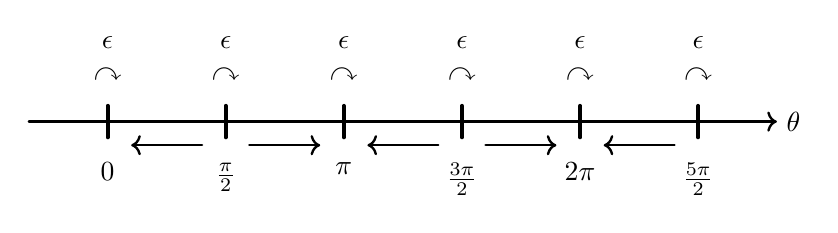
\begin{tikzpicture}[line join = round, line cap = round]
		\coordinate (a) at (0.0,0.8);
		\coordinate (b) at (0.0,-0.4);
		\coordinate (br) at (0.3,-0.3);
		\coordinate (bl) at (-0.3,-0.3);
		\coordinate (l) at (-1,0);
		\coordinate (m0) at (0,0);
		\tick{(m0)};
		\coordinate[label=above:{$\epsilon$}, label=below:{$\curvearrowright$}] (m0a) at ($(m0) + (a)$);
		\coordinate[label=below:{$0$}] (m0b) at ($(m0) + (b)$);
		\coordinate (m0br) at ($(m0) + (br)$);
		\coordinate (m1) at (1.5,0);
		\tick{(m1)};
		\coordinate[label=above:{$\epsilon$}, label=below:{$\curvearrowright$}] (m1a) at ($(m1) + (a)$);
		\coordinate[label=below:{$\frac{\pi}{2}$}] (m1b) at ($(m1) + (b)$);
		\coordinate (m1bl) at ($(m1) + (bl)$);
		\coordinate (m1br) at ($(m1) + (br)$);
		\coordinate (m2) at (3,0);
		\tick{(m2)};
		\coordinate[label=above:{$\epsilon$}, label=below:{$\curvearrowright$}] (m2a) at ($(m2) + (a)$);
		\coordinate[label=below:{$\pi$}] (m2b) at ($(m2) + (b)$);
		\coordinate (m2bl) at ($(m2) + (bl)$);
		\coordinate (m2br) at ($(m2) + (br)$);
		\coordinate (m3) at (4.5,0);
		\tick{(m3)};
		\coordinate[label=above:{$\epsilon$}, label=below:{$\curvearrowright$}] (m3a) at ($(m3) + (a)$);
		\coordinate[label=below:{$\frac{3\pi}{2}$}] (m3b) at ($(m3) + (b)$);
		\coordinate (m3bl) at ($(m3) + (bl)$);
		\coordinate (m3br) at ($(m3) + (br)$);
		\coordinate (m4) at (6.0,0);
		\tick{(m4)};
		\coordinate[label=above:{$\epsilon$}, label=below:{$\curvearrowright$}] (m4a) at ($(m4) + (a)$);
		\coordinate[label=below:{$2\pi$}] (m4b) at ($(m4) + (b)$);
		\coordinate (m4bl) at ($(m4) + (bl)$);
		\coordinate (m4br) at ($(m4) + (br)$);
		\coordinate (m5) at (7.5,0);
		\tick{(m5)};
		\coordinate[label=above:{$\epsilon$}, label=below:{$\curvearrowright$}] (m5a) at ($(m5) + (a)$);
		\coordinate[label=below:{$\frac{5\pi}{2}$}] (m5b) at ($(m5) + (b)$);
		\coordinate (m5bl) at ($(m5) + (bl)$);
		\coordinate[label=right:{$\theta$}] (r) at (8.5,0);
		\draw [->,color=black,line width=0.3mm] (l)--(r);
		\draw [->,color=black,line width=0.3mm] (m1bl)--(m0br);
		\draw [->,color=black,line width=0.3mm] (m1br)--(m2bl);
		\draw [->,color=black,line width=0.3mm] (m3bl)--(m2br);
		\draw [->,color=black,line width=0.3mm] (m3br)--(m4bl);
		\draw [->,color=black,line width=0.3mm] (m5bl)--(m4br);
		\end{tikzpicture}
		\caption{\it The dynamics of $\theta_n$ on the real line in the unbalanced case where $\mathbb{E}(\log(\kappa_n)) < 0$. This induces local drifts indicated by the arrows below the axis.}
\label{fig:theta-unbalanced}
	\end{center}
\end{figure}
%
%
\begin{gather}\label{ineq:slower-faster-unbalanced}
	\frac{1}{\mathbb{E}(\widehat{T}_1^\epsilon) + \mathbb{E}(\widehat{T}_2^\epsilon)} 
	\;\leq\; 
	\lim_{N \to \infty} \frac{1}{N}\frac{\mathbb{E}(\theta^\epsilon_N)}{\pi} 
	\;\leq\; 
	\frac{1}{\mathbb{E}(\widetilde{T}_1^\epsilon) + \mathbb{E}(\widetilde{T}_2^\epsilon)}\;,
\end{gather}
%
for which again two independent and identically distributed families of random dynamical processes $\widehat{x}^\epsilon_k=(\widehat{x}^\epsilon_{k,n})_{n\geq 0}$ and $\widetilde{x}^\epsilon_k=(\widetilde{x}^\epsilon_{k,n})_{n\geq 0}$ can be constructed. This is possible on $[0,\infty)$ due to the assumption that $\log(\kappa_\sigma)$ is compactly supported and due to the validity of the estimates on the action of $Q^\epsilon$ provided in Lemma~\eqref{lemma:Q-lower} and Lemma~\ref{lemma:Q-upper}.  As argued further on, the contribution of $\widehat{T}^\epsilon_1$ will dominate that of $\widehat{T}^\epsilon_2$ for small $\epsilon$ (see the arrows in Fig.~\ref{fig:theta-unbalanced} indicating the drifts), and the same holds for $\widetilde{T}^\epsilon_1$ and $\widetilde{T}^\epsilon_2$. Applying logarithmic transformations similar to $\widehat{f}$ and $\widetilde{f}$ to the processes $\widehat{x}^\epsilon_1$ and $\widetilde{x}^\epsilon_1$, one can obtain exactly the same processes $\widehat{y}$ and $\widetilde{y}$ as in~\eqref{eq:y-slower} and~\eqref{eq:y-faster} (again for $n$ smaller than some stopping time similar to $\widehat{T}_{-,+}$ or $\widetilde{T}_{-,+}$ respectively). Also the calculations leading to~\eqref{ineq:slower} and~\eqref{ineq:faster} remain valid. For $\lambda$ (and hence $\epsilon$) small enough, the above random walks starting at $0$ contain a drift in the negative direction. As in the previous section, each expectation in~\eqref{ineq:slower-faster-unbalanced} can be found by applying the optional stopping theorem to two martingales, which in the present situation are $\widehat{y}_n - n\mathbb{E}(\chi)$ and $e^{C_0\nu\widehat{y}_n}$ (and similarly with tildes instead of hats, compare with the previous section). Now introduce the quantities
%
\begin{align*}
	\widehat{y}'''_- &\,:=\, \tfrac{1}{C_0\nu}\log\Big(\mathbb{E}\big(e^{C_0\nu\widehat{y}_{\widehat{T}_{-,+}}} \,\big|\, \widehat{y}_{\widehat{T}_{-,+}} \leq \widehat{y}_-\big)\Big)\,,&\;\;& \widetilde{y}'''_- \,:=\, \tfrac{1}{C_0\nu}\log\Big(\mathbb{E}\big(e^{C_0\nu\widetilde{y}_{\widetilde{T}_{-,+}}} \,\big|\, \widetilde{y}_{\widetilde{T}_{-,+}} \leq \widetilde{y}_-\big)\Big)\,,\\
	\widehat{y}'''_+ &\,:=\, \tfrac{1}{C_0\nu}\log\Big(\mathbb{E}\big(e^{C_0\nu\widehat{y}_{\widehat{T}_{-,+}}} \,\big|\, \widehat{y}_{\widehat{T}_{-,+}} \geq \widehat{y}_+\big)\Big)\,,&\;\;& \widetilde{y}'''_+ \,:=\, \tfrac{1}{C_0\nu}\log\Big(\mathbb{E}\big(e^{C_0\nu\widetilde{y}_{\widetilde{T}_{-,+}}} \,\big|\, \widetilde{y}_{\widetilde{T}_{-,+}} \geq \widetilde{y}_+\big)\Big)\,.
\end{align*}
%
One has $\widehat{y}'''_- \in \left[\widehat{y}_--1,\widehat{y}_-\right]$, $\widetilde{y}'''_- \in \left[\widetilde{y}_--1,\widetilde{y}_-\right]$, $\widehat{y}'''_+ \leq \widehat{y}_+ + 1$ and $\widetilde{y}'''_+ \geq \widetilde{y}_+$. Applying the optional stopping theorem to the two martingales mentioned before now yields
%
\begin{gather}
\label{eq:unbalanced}
\mathbb{E}(\widehat{T}_1) 
\;=\; 
\left(1 + \frac{C_0\,\widehat{y}'_-}{\mathbb{E}(\log(\kappa_0))}\right)\,\frac{e^{C_0\nu\widehat{y}'''_+}-e^{C_0\nu\widehat{y}'''_-}}{1-e^{C_0\nu\widehat{y}'''_-}}\, +\, \frac{C_0\,(\widehat{y}'_+ - \widehat{y}'_-)}{\mathbb{E}(\log(\kappa_0))}\, +\, 2
\,,
\end{gather}
%
and again similarly with tildes instead of hats. The limits of Lemma~\ref{lemma:slower-y-lims} and~\ref{lemma:faster-y-lims} then show that the expressions on the two r.h.s. diverge proportionally to $\epsilon^{-\nu}$ for $\epsilon\downarrow 0$. Note that the drift originating from $\mathbb{E}(\log(\kappa_n)) < 0$ leads to a dynamics going faster through $\overline{\mathbb{R}}\backslash[0,\infty)$ on average than in the balanced case $\mathbb{E}(\log(\kappa_n)) = 0$. Hence, $\widehat{T}^\epsilon_2$ and $\widetilde{T}^\epsilon_2$ can at most diverge proportionally to $(-\log(\epsilon))^2$, namely as in the balanced case. Therefore the power law of~\eqref{eq:unbalanced} will dominate this contribution in~\eqref{ineq:slower-faster-unbalanced}. After some algebra, one concludes that
%
$$
\frac{\mathbb{E}(\log(\tfrac{1}{\kappa_0}))\left(1 - (1+e^{-2C_0})^{-\frac{\nu}{2}}\right)}{2\,\mathbb{E}(\log(\tfrac{1}{\kappa_0})) + 2\,C_0 + \log(1+e^{-2C_0})} 
\;\leq\; 
\EM(L_\sigma)\,\frac{|\mathcal{N}(\epsilon) - \mathcal{N}(0)|}{|\epsilon|^{\nu}} 
\;\leq\; 
\frac{\mathbb{E}(\log(\tfrac{1}{\kappa_0}))e^{C_0\nu}\left(1 - e^{-2C_0\nu}\right)}{2\,\mathbb{E}(\log(\tfrac{1}{\kappa_0})) + 1}
$$
%
for $\epsilon$ small enough and $E_c=0$. As already stress in Section~\ref{sec-Hopping}, this is a considerable strengthening of the main result of~\cite{DS}.

\vspace{.2cm}

\noindent {\bf Acknowledgements:} This work was supported by the DFG grant SCHU 1358/6-2 and the Chilean grant FONDECYT 1201836. 


%%%%%%%%%%%%%%%%%%%%%%%%%%%%%%%%%%%%%%%%%%%%%
\begin{thebibliography}{99}
\bibliographystyle{unsrt}


\bibitem{BL} P.~Bougerol, J.~Lacroix, {\sl Products of Random Matrices with Applications to Schr{\"o}dinger Operators}, (Birkh{\"a}user, Boston, 1985).

\bibitem{DS} F.~Dorsch, H.~Schulz-Baldes, {\sl Pseudo-gaps for random hopping models},
J. Physics A: Mathematical and Theoretical {\bf 53}, 185201 (2020).

\bibitem{DKS} M.~Drabkin, W.~Kirsch, H.~Schulz-Baldes, {\sl Transport in the random Kronig-Penney model}, J. Math. Phys. {\bf 53}, 122109 (2012).

\bibitem{DWP} D.~H.~Dunlap, H.~L.~Wu, P.~W.~Phillips, {\sl Absence of localization in a random-dimer model}, Phys. Rev. Lett.{\bf 65}, 88-91 (1990).

\bibitem{DC} V.~Dwivedi, V.~Chua, {\sl Of Bulk and Boundaries: Generalized Transfer Matrices for Tight-Binding Models}, Phys. Rev. {\bf B 93}, 134304 (2016).

\bibitem{Eth} S.~N.~Ethier, {\sl The doctrine of chances: probabilistic aspects of gambling}, (Springer, Berlin, 2010).

\bibitem{GSh} G.~Graf, J.~Shapiro, {\sl The bulk-edge correspondence for disordered chiral chains}, Commun. Math. Phys. {\bf 363}, 829-846 (2018).

\bibitem{GS} G.~Grimmett, D.~Stirzaker, {\sl Probability and random processes}, (Oxford University Press, 2001).

\bibitem{JSS} S.~Jitomirskaya, H.~Schulz-Baldes, G.~Stolz, {\sl Delocalization in random polymer models},
Commun. Math. Phys. {\bf 233}, 27-48  (2003).

\bibitem{Luc} J.~M.~Luck, {\sl  Systemes d\'esordonn\'es unidimensionnels}, (CEA, Sacley, 1992).

\bibitem{MSHP}
I.~Mondragon-Shem, J.~Song, T.~L. Hughes,  E.~Prodan, {\sl  Topological criticality in the chiral-symmetric AIII class at strong  disorder}, Phys. Rev. Lett. {\bf 113},  046802 (2014).

\bibitem{MPS}
P.~M\"uller, L.~Pastur, R.~Schulte, {\sl How Much Delocalisation is Needed for an Enhanced Area Law of the Entanglement Entropy?}, Commun. Math. Phys. {\bf 376}, 649-679 (2020).

\bibitem{PF} L. Pastur, A. Figotin, {\sl Spectra of Random and Almost-Periodic Operators}, (Springer, Berlin, 1992).

\bibitem{PS}
E.~Prodan, H.~Schulz-Baldes, {\sl Bulk and Boundary Invariants for Complex Topological Insulators: From $K$-Theory to Physics}, (Springer International, Cham, 2016).

\bibitem{Sad} C.~Sadel, {\sl Spectral theory of one-channel operators and application to absolutely continuous spectrum for Anderson type models}, J. Functional Analysis {\bf 274}, 2205-2244 (2018).

\bibitem{ST} H.~Schulz-Baldes, T.~Stoiber, {\sl Harmonic analysis in operator algebras and its applications to index theory and topological solid state systems}, (Springer International, Cham, 2022).

\bibitem{SB} H.~Schulz-Baldes, {\sl Reduced transfer operators for singular difference equations}, J.  Difference Eq. Appl. {\bf 28}, 1492-1506 (2022).

\bibitem{Sh} J. Shaprio, {\sl Incomplete localization for disordered chiral strips}, {\tt arXiv:2108.10978}.

\bibitem{SSH} W.~P.~Su, J.~R.~Schrieffer, A.~J.~Heeger, {\sl Soliton excitations in polyacetylene}, Phys. Rev. {\bf B 22}, 2099-2111 (1980).

\end{thebibliography}

\end{document}

